\section{Testy klasycznych regulatorów PID i DMC}
\label{lab:zad3}

Regulatory PID oraz DMC opracowane na laboratorium 1 dla obiektu liniowego
zostały przetestowane dla obiektu nieliniowego. Ustawiono trajektorię zmian
sygnałów zadanych $T= 39.4, 44.4, 54.4 39.4$


\subsection{Klasyczny algorytm PID}
\label{lab:zad3:PID}

\begin{figure}[H] 
   \centering
   % This file was created by matlab2tikz.
%
\definecolor{mycolor1}{rgb}{0.00000,0.44700,0.74100}%
\definecolor{mycolor2}{rgb}{0.85000,0.32500,0.09800}%
%
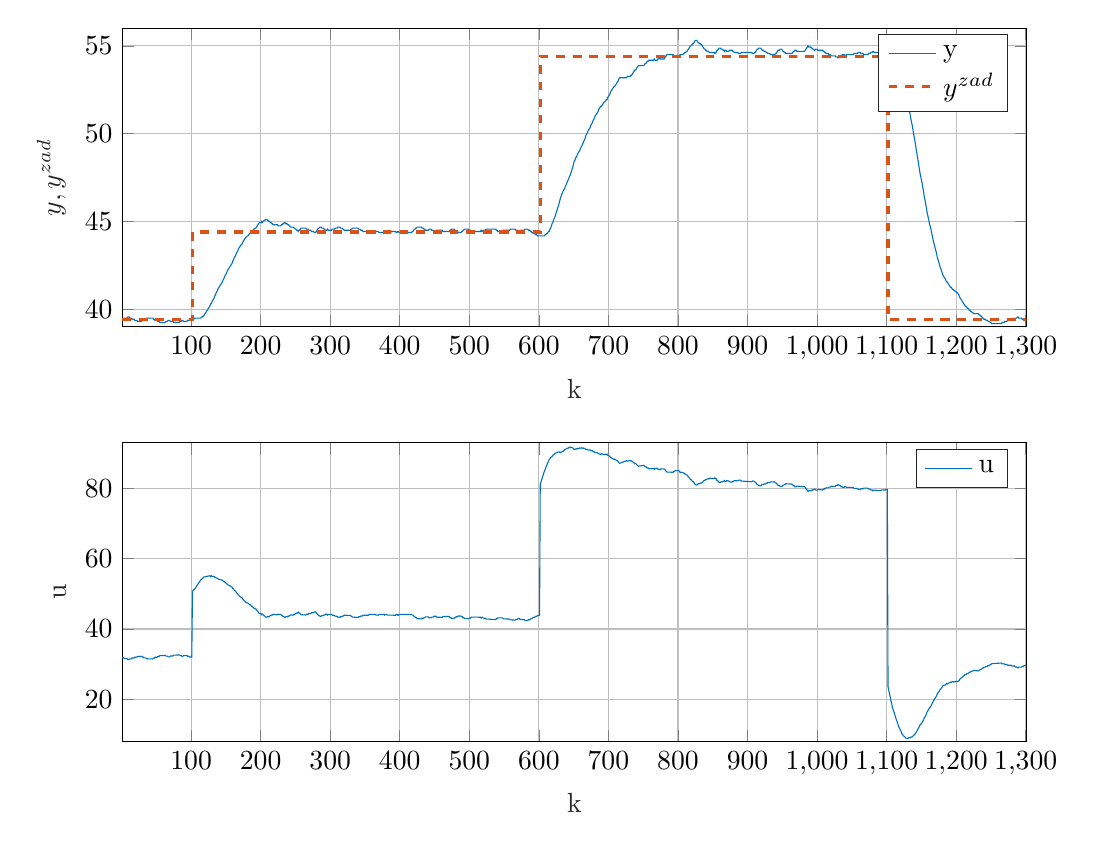
\begin{tikzpicture}

\begin{axis}[%
width=4.521in,
height=1.493in,
at={(0.758in,2.554in)},
scale only axis,
xmin=1,
xmax=1301,
xlabel style={font=\color{white!15!black}},
xlabel={k},
ymin=39,
ymax=56,
ylabel style={font=\color{white!15!black}},
ylabel={$\text{y, y}^{\text{zad}}$},
axis background/.style={fill=white},
xmajorgrids,
ymajorgrids,
legend style={legend cell align=left, align=left, draw=white!15!black}
]
\addplot [color=mycolor1]
  table[row sep=crcr]{%
1	39.43\\
2	39.43\\
3	39.43\\
4	39.5\\
5	39.5\\
6	39.5\\
7	39.5\\
8	39.5\\
9	39.56\\
10	39.56\\
11	39.56\\
12	39.5\\
13	39.5\\
14	39.5\\
15	39.43\\
16	39.43\\
17	39.43\\
18	39.43\\
19	39.37\\
20	39.37\\
21	39.37\\
22	39.37\\
23	39.31\\
24	39.31\\
25	39.31\\
26	39.31\\
27	39.31\\
28	39.31\\
29	39.31\\
30	39.37\\
31	39.37\\
32	39.43\\
33	39.43\\
34	39.43\\
35	39.43\\
36	39.5\\
37	39.5\\
38	39.5\\
39	39.5\\
40	39.5\\
41	39.5\\
42	39.5\\
43	39.5\\
44	39.5\\
45	39.5\\
46	39.43\\
47	39.43\\
48	39.37\\
49	39.37\\
50	39.37\\
51	39.37\\
52	39.31\\
53	39.31\\
54	39.31\\
55	39.25\\
56	39.25\\
57	39.25\\
58	39.25\\
59	39.25\\
60	39.25\\
61	39.25\\
62	39.25\\
63	39.25\\
64	39.31\\
65	39.31\\
66	39.31\\
67	39.37\\
68	39.37\\
69	39.37\\
70	39.31\\
71	39.31\\
72	39.31\\
73	39.31\\
74	39.31\\
75	39.25\\
76	39.25\\
77	39.25\\
78	39.25\\
79	39.25\\
80	39.25\\
81	39.25\\
82	39.25\\
83	39.25\\
84	39.31\\
85	39.31\\
86	39.31\\
87	39.37\\
88	39.37\\
89	39.31\\
90	39.31\\
91	39.31\\
92	39.31\\
93	39.31\\
94	39.31\\
95	39.37\\
96	39.37\\
97	39.37\\
98	39.43\\
99	39.43\\
100	39.43\\
101	39.43\\
102	39.43\\
103	39.43\\
104	39.43\\
105	39.5\\
106	39.5\\
107	39.5\\
108	39.5\\
109	39.5\\
110	39.5\\
111	39.5\\
112	39.5\\
113	39.5\\
114	39.5\\
115	39.56\\
116	39.56\\
117	39.62\\
118	39.62\\
119	39.68\\
120	39.75\\
121	39.81\\
122	39.87\\
123	39.93\\
124	40\\
125	40.06\\
126	40.12\\
127	40.18\\
128	40.31\\
129	40.31\\
130	40.43\\
131	40.5\\
132	40.56\\
133	40.62\\
134	40.75\\
135	40.81\\
136	40.93\\
137	41\\
138	41.06\\
139	41.18\\
140	41.25\\
141	41.31\\
142	41.37\\
143	41.43\\
144	41.5\\
145	41.56\\
146	41.68\\
147	41.75\\
148	41.81\\
149	41.93\\
150	42\\
151	42.06\\
152	42.18\\
153	42.25\\
154	42.31\\
155	42.37\\
156	42.43\\
157	42.5\\
158	42.56\\
159	42.62\\
160	42.75\\
161	42.81\\
162	42.93\\
163	43\\
164	43.06\\
165	43.18\\
166	43.25\\
167	43.31\\
168	43.43\\
169	43.5\\
170	43.56\\
171	43.62\\
172	43.68\\
173	43.68\\
174	43.81\\
175	43.87\\
176	43.93\\
177	44\\
178	44.06\\
179	44.12\\
180	44.12\\
181	44.18\\
182	44.18\\
183	44.25\\
184	44.31\\
185	44.31\\
186	44.37\\
187	44.43\\
188	44.43\\
189	44.5\\
190	44.56\\
191	44.56\\
192	44.62\\
193	44.62\\
194	44.68\\
195	44.75\\
196	44.81\\
197	44.87\\
198	44.93\\
199	44.93\\
200	44.93\\
201	45\\
202	44.93\\
203	45\\
204	45\\
205	45.06\\
206	45.06\\
207	45.12\\
208	45.12\\
209	45.12\\
210	45.06\\
211	45.06\\
212	45\\
213	45\\
214	44.93\\
215	44.93\\
216	44.87\\
217	44.87\\
218	44.81\\
219	44.81\\
220	44.81\\
221	44.81\\
222	44.81\\
223	44.81\\
224	44.81\\
225	44.75\\
226	44.75\\
227	44.75\\
228	44.75\\
229	44.75\\
230	44.81\\
231	44.81\\
232	44.87\\
233	44.87\\
234	44.93\\
235	44.93\\
236	44.87\\
237	44.87\\
238	44.87\\
239	44.81\\
240	44.81\\
241	44.75\\
242	44.75\\
243	44.68\\
244	44.68\\
245	44.68\\
246	44.68\\
247	44.68\\
248	44.62\\
249	44.62\\
250	44.56\\
251	44.56\\
252	44.5\\
253	44.5\\
254	44.43\\
255	44.5\\
256	44.5\\
257	44.56\\
258	44.62\\
259	44.62\\
260	44.62\\
261	44.62\\
262	44.62\\
263	44.62\\
264	44.62\\
265	44.62\\
266	44.56\\
267	44.56\\
268	44.56\\
269	44.5\\
270	44.5\\
271	44.5\\
272	44.5\\
273	44.43\\
274	44.43\\
275	44.43\\
276	44.43\\
277	44.37\\
278	44.37\\
279	44.37\\
280	44.43\\
281	44.5\\
282	44.56\\
283	44.62\\
284	44.62\\
285	44.68\\
286	44.68\\
287	44.68\\
288	44.62\\
289	44.62\\
290	44.62\\
291	44.56\\
292	44.56\\
293	44.5\\
294	44.5\\
295	44.5\\
296	44.56\\
297	44.5\\
298	44.5\\
299	44.5\\
300	44.5\\
301	44.5\\
302	44.5\\
303	44.56\\
304	44.56\\
305	44.56\\
306	44.56\\
307	44.62\\
308	44.62\\
309	44.62\\
310	44.62\\
311	44.68\\
312	44.68\\
313	44.68\\
314	44.68\\
315	44.62\\
316	44.62\\
317	44.62\\
318	44.56\\
319	44.56\\
320	44.5\\
321	44.5\\
322	44.5\\
323	44.5\\
324	44.5\\
325	44.5\\
326	44.5\\
327	44.5\\
328	44.5\\
329	44.5\\
330	44.56\\
331	44.56\\
332	44.62\\
333	44.62\\
334	44.62\\
335	44.62\\
336	44.62\\
337	44.62\\
338	44.62\\
339	44.62\\
340	44.62\\
341	44.56\\
342	44.56\\
343	44.56\\
344	44.5\\
345	44.5\\
346	44.5\\
347	44.43\\
348	44.43\\
349	44.43\\
350	44.43\\
351	44.43\\
352	44.43\\
353	44.43\\
354	44.43\\
355	44.43\\
356	44.37\\
357	44.37\\
358	44.37\\
359	44.37\\
360	44.37\\
361	44.37\\
362	44.37\\
363	44.37\\
364	44.37\\
365	44.37\\
366	44.43\\
367	44.43\\
368	44.43\\
369	44.43\\
370	44.37\\
371	44.37\\
372	44.37\\
373	44.37\\
374	44.37\\
375	44.37\\
376	44.37\\
377	44.37\\
378	44.43\\
379	44.37\\
380	44.37\\
381	44.37\\
382	44.43\\
383	44.43\\
384	44.43\\
385	44.43\\
386	44.43\\
387	44.43\\
388	44.43\\
389	44.43\\
390	44.43\\
391	44.43\\
392	44.43\\
393	44.43\\
394	44.43\\
395	44.37\\
396	44.37\\
397	44.43\\
398	44.43\\
399	44.37\\
400	44.37\\
401	44.37\\
402	44.37\\
403	44.37\\
404	44.37\\
405	44.37\\
406	44.37\\
407	44.37\\
408	44.37\\
409	44.37\\
410	44.37\\
411	44.37\\
412	44.37\\
413	44.37\\
414	44.37\\
415	44.37\\
416	44.37\\
417	44.37\\
418	44.43\\
419	44.43\\
420	44.5\\
421	44.56\\
422	44.56\\
423	44.62\\
424	44.62\\
425	44.68\\
426	44.68\\
427	44.68\\
428	44.68\\
429	44.68\\
430	44.68\\
431	44.68\\
432	44.62\\
433	44.62\\
434	44.62\\
435	44.56\\
436	44.56\\
437	44.5\\
438	44.5\\
439	44.5\\
440	44.5\\
441	44.5\\
442	44.56\\
443	44.56\\
444	44.56\\
445	44.56\\
446	44.5\\
447	44.5\\
448	44.5\\
449	44.43\\
450	44.43\\
451	44.43\\
452	44.43\\
453	44.5\\
454	44.5\\
455	44.5\\
456	44.5\\
457	44.5\\
458	44.5\\
459	44.5\\
460	44.5\\
461	44.5\\
462	44.43\\
463	44.43\\
464	44.43\\
465	44.43\\
466	44.43\\
467	44.43\\
468	44.43\\
469	44.43\\
470	44.43\\
471	44.43\\
472	44.5\\
473	44.5\\
474	44.56\\
475	44.56\\
476	44.56\\
477	44.56\\
478	44.56\\
479	44.5\\
480	44.5\\
481	44.43\\
482	44.43\\
483	44.43\\
484	44.37\\
485	44.37\\
486	44.37\\
487	44.37\\
488	44.37\\
489	44.43\\
490	44.43\\
491	44.5\\
492	44.5\\
493	44.56\\
494	44.56\\
495	44.56\\
496	44.56\\
497	44.56\\
498	44.56\\
499	44.56\\
500	44.5\\
501	44.5\\
502	44.5\\
503	44.43\\
504	44.43\\
505	44.43\\
506	44.43\\
507	44.43\\
508	44.43\\
509	44.43\\
510	44.43\\
511	44.43\\
512	44.43\\
513	44.43\\
514	44.43\\
515	44.43\\
516	44.43\\
517	44.5\\
518	44.43\\
519	44.43\\
520	44.5\\
521	44.5\\
522	44.5\\
523	44.5\\
524	44.56\\
525	44.56\\
526	44.56\\
527	44.56\\
528	44.56\\
529	44.56\\
530	44.56\\
531	44.56\\
532	44.56\\
533	44.56\\
534	44.56\\
535	44.56\\
536	44.56\\
537	44.56\\
538	44.56\\
539	44.5\\
540	44.5\\
541	44.43\\
542	44.43\\
543	44.43\\
544	44.43\\
545	44.43\\
546	44.43\\
547	44.43\\
548	44.43\\
549	44.5\\
550	44.5\\
551	44.5\\
552	44.5\\
553	44.5\\
554	44.5\\
555	44.5\\
556	44.5\\
557	44.5\\
558	44.5\\
559	44.56\\
560	44.56\\
561	44.56\\
562	44.56\\
563	44.56\\
564	44.56\\
565	44.56\\
566	44.56\\
567	44.5\\
568	44.5\\
569	44.5\\
570	44.43\\
571	44.43\\
572	44.43\\
573	44.5\\
574	44.5\\
575	44.5\\
576	44.5\\
577	44.5\\
578	44.5\\
579	44.5\\
580	44.56\\
581	44.56\\
582	44.56\\
583	44.56\\
584	44.56\\
585	44.5\\
586	44.5\\
587	44.5\\
588	44.43\\
589	44.43\\
590	44.37\\
591	44.37\\
592	44.31\\
593	44.31\\
594	44.31\\
595	44.25\\
596	44.25\\
597	44.25\\
598	44.18\\
599	44.18\\
600	44.18\\
601	44.18\\
602	44.18\\
603	44.18\\
604	44.18\\
605	44.18\\
606	44.18\\
607	44.18\\
608	44.18\\
609	44.25\\
610	44.25\\
611	44.31\\
612	44.31\\
613	44.37\\
614	44.43\\
615	44.43\\
616	44.56\\
617	44.62\\
618	44.75\\
619	44.87\\
620	44.93\\
621	45.06\\
622	45.18\\
623	45.25\\
624	45.37\\
625	45.5\\
626	45.62\\
627	45.75\\
628	45.87\\
629	46\\
630	46.18\\
631	46.31\\
632	46.43\\
633	46.56\\
634	46.62\\
635	46.75\\
636	46.81\\
637	46.87\\
638	47\\
639	47.06\\
640	47.18\\
641	47.25\\
642	47.37\\
643	47.43\\
644	47.56\\
645	47.62\\
646	47.75\\
647	47.87\\
648	48\\
649	48.12\\
650	48.31\\
651	48.43\\
652	48.5\\
653	48.62\\
654	48.68\\
655	48.75\\
656	48.87\\
657	48.93\\
658	49\\
659	49.06\\
660	49.18\\
661	49.25\\
662	49.31\\
663	49.43\\
664	49.5\\
665	49.62\\
666	49.68\\
667	49.81\\
668	49.93\\
669	50\\
670	50.06\\
671	50.18\\
672	50.25\\
673	50.31\\
674	50.37\\
675	50.5\\
676	50.56\\
677	50.62\\
678	50.75\\
679	50.81\\
680	50.93\\
681	51\\
682	51.06\\
683	51.12\\
684	51.18\\
685	51.25\\
686	51.37\\
687	51.43\\
688	51.5\\
689	51.56\\
690	51.56\\
691	51.62\\
692	51.68\\
693	51.75\\
694	51.81\\
695	51.81\\
696	51.87\\
697	51.93\\
698	51.93\\
699	52.06\\
700	52.12\\
701	52.18\\
702	52.25\\
703	52.37\\
704	52.43\\
705	52.5\\
706	52.56\\
707	52.62\\
708	52.68\\
709	52.68\\
710	52.75\\
711	52.81\\
712	52.87\\
713	52.93\\
714	53\\
715	53.12\\
716	53.18\\
717	53.18\\
718	53.18\\
719	53.18\\
720	53.18\\
721	53.18\\
722	53.18\\
723	53.18\\
724	53.18\\
725	53.18\\
726	53.18\\
727	53.25\\
728	53.25\\
729	53.25\\
730	53.25\\
731	53.25\\
732	53.31\\
733	53.31\\
734	53.37\\
735	53.43\\
736	53.5\\
737	53.56\\
738	53.62\\
739	53.62\\
740	53.68\\
741	53.75\\
742	53.81\\
743	53.87\\
744	53.87\\
745	53.87\\
746	53.87\\
747	53.87\\
748	53.87\\
749	53.87\\
750	53.87\\
751	53.87\\
752	53.93\\
753	54\\
754	54\\
755	54.06\\
756	54.12\\
757	54.12\\
758	54.18\\
759	54.18\\
760	54.18\\
761	54.18\\
762	54.18\\
763	54.18\\
764	54.18\\
765	54.18\\
766	54.25\\
767	54.18\\
768	54.18\\
769	54.18\\
770	54.18\\
771	54.25\\
772	54.25\\
773	54.31\\
774	54.31\\
775	54.25\\
776	54.25\\
777	54.25\\
778	54.25\\
779	54.25\\
780	54.25\\
781	54.31\\
782	54.37\\
783	54.43\\
784	54.5\\
785	54.5\\
786	54.5\\
787	54.5\\
788	54.5\\
789	54.5\\
790	54.5\\
791	54.5\\
792	54.5\\
793	54.5\\
794	54.43\\
795	54.43\\
796	54.37\\
797	54.37\\
798	54.37\\
799	54.37\\
800	54.37\\
801	54.37\\
802	54.43\\
803	54.5\\
804	54.5\\
805	54.5\\
806	54.5\\
807	54.5\\
808	54.56\\
809	54.56\\
810	54.62\\
811	54.62\\
812	54.68\\
813	54.68\\
814	54.75\\
815	54.81\\
816	54.87\\
817	54.93\\
818	55\\
819	55\\
820	55.06\\
821	55.12\\
822	55.12\\
823	55.18\\
824	55.25\\
825	55.31\\
826	55.31\\
827	55.31\\
828	55.25\\
829	55.18\\
830	55.18\\
831	55.12\\
832	55.12\\
833	55.06\\
834	55.06\\
835	55\\
836	54.93\\
837	54.87\\
838	54.81\\
839	54.81\\
840	54.75\\
841	54.75\\
842	54.68\\
843	54.68\\
844	54.68\\
845	54.62\\
846	54.62\\
847	54.62\\
848	54.62\\
849	54.62\\
850	54.62\\
851	54.62\\
852	54.62\\
853	54.56\\
854	54.62\\
855	54.62\\
856	54.75\\
857	54.75\\
858	54.81\\
859	54.87\\
860	54.87\\
861	54.87\\
862	54.81\\
863	54.81\\
864	54.81\\
865	54.75\\
866	54.75\\
867	54.68\\
868	54.75\\
869	54.75\\
870	54.68\\
871	54.68\\
872	54.68\\
873	54.68\\
874	54.75\\
875	54.75\\
876	54.75\\
877	54.75\\
878	54.75\\
879	54.68\\
880	54.68\\
881	54.62\\
882	54.62\\
883	54.62\\
884	54.62\\
885	54.62\\
886	54.62\\
887	54.56\\
888	54.56\\
889	54.56\\
890	54.56\\
891	54.62\\
892	54.62\\
893	54.62\\
894	54.62\\
895	54.62\\
896	54.62\\
897	54.62\\
898	54.62\\
899	54.62\\
900	54.62\\
901	54.62\\
902	54.62\\
903	54.62\\
904	54.62\\
905	54.62\\
906	54.62\\
907	54.56\\
908	54.56\\
909	54.56\\
910	54.62\\
911	54.62\\
912	54.68\\
913	54.75\\
914	54.81\\
915	54.81\\
916	54.87\\
917	54.87\\
918	54.87\\
919	54.87\\
920	54.81\\
921	54.75\\
922	54.75\\
923	54.75\\
924	54.68\\
925	54.68\\
926	54.68\\
927	54.62\\
928	54.62\\
929	54.56\\
930	54.56\\
931	54.56\\
932	54.56\\
933	54.5\\
934	54.5\\
935	54.5\\
936	54.5\\
937	54.5\\
938	54.5\\
939	54.5\\
940	54.56\\
941	54.56\\
942	54.62\\
943	54.68\\
944	54.75\\
945	54.75\\
946	54.75\\
947	54.81\\
948	54.81\\
949	54.81\\
950	54.75\\
951	54.68\\
952	54.68\\
953	54.62\\
954	54.62\\
955	54.56\\
956	54.56\\
957	54.56\\
958	54.56\\
959	54.56\\
960	54.56\\
961	54.56\\
962	54.56\\
963	54.56\\
964	54.56\\
965	54.62\\
966	54.68\\
967	54.68\\
968	54.75\\
969	54.75\\
970	54.75\\
971	54.68\\
972	54.68\\
973	54.68\\
974	54.68\\
975	54.68\\
976	54.68\\
977	54.68\\
978	54.68\\
979	54.68\\
980	54.68\\
981	54.68\\
982	54.68\\
983	54.75\\
984	54.81\\
985	54.87\\
986	54.93\\
987	55\\
988	54.93\\
989	54.93\\
990	54.93\\
991	54.93\\
992	54.87\\
993	54.87\\
994	54.81\\
995	54.81\\
996	54.75\\
997	54.75\\
998	54.81\\
999	54.81\\
1000	54.81\\
1001	54.75\\
1002	54.75\\
1003	54.75\\
1004	54.75\\
1005	54.75\\
1006	54.75\\
1007	54.75\\
1008	54.75\\
1009	54.68\\
1010	54.68\\
1011	54.62\\
1012	54.62\\
1013	54.56\\
1014	54.56\\
1015	54.56\\
1016	54.56\\
1017	54.5\\
1018	54.5\\
1019	54.5\\
1020	54.43\\
1021	54.43\\
1022	54.43\\
1023	54.43\\
1024	54.43\\
1025	54.43\\
1026	54.43\\
1027	54.37\\
1028	54.37\\
1029	54.37\\
1030	54.31\\
1031	54.31\\
1032	54.37\\
1033	54.37\\
1034	54.43\\
1035	54.43\\
1036	54.5\\
1037	54.5\\
1038	54.5\\
1039	54.5\\
1040	54.43\\
1041	54.43\\
1042	54.5\\
1043	54.5\\
1044	54.5\\
1045	54.5\\
1046	54.5\\
1047	54.5\\
1048	54.5\\
1049	54.5\\
1050	54.5\\
1051	54.5\\
1052	54.5\\
1053	54.56\\
1054	54.56\\
1055	54.56\\
1056	54.56\\
1057	54.56\\
1058	54.56\\
1059	54.62\\
1060	54.62\\
1061	54.62\\
1062	54.62\\
1063	54.56\\
1064	54.56\\
1065	54.56\\
1066	54.56\\
1067	54.5\\
1068	54.5\\
1069	54.5\\
1070	54.5\\
1071	54.5\\
1072	54.5\\
1073	54.5\\
1074	54.56\\
1075	54.56\\
1076	54.56\\
1077	54.62\\
1078	54.62\\
1079	54.62\\
1080	54.68\\
1081	54.68\\
1082	54.62\\
1083	54.62\\
1084	54.62\\
1085	54.62\\
1086	54.62\\
1087	54.62\\
1088	54.62\\
1089	54.62\\
1090	54.62\\
1091	54.62\\
1092	54.62\\
1093	54.56\\
1094	54.56\\
1095	54.56\\
1096	54.56\\
1097	54.56\\
1098	54.56\\
1099	54.5\\
1100	54.5\\
1101	54.5\\
1102	54.56\\
1103	54.56\\
1104	54.56\\
1105	54.56\\
1106	54.62\\
1107	54.56\\
1108	54.56\\
1109	54.5\\
1110	54.43\\
1111	54.31\\
1112	54.25\\
1113	54.18\\
1114	54.12\\
1115	54\\
1116	53.93\\
1117	53.87\\
1118	53.75\\
1119	53.62\\
1120	53.5\\
1121	53.37\\
1122	53.31\\
1123	53.12\\
1124	53\\
1125	52.81\\
1126	52.62\\
1127	52.5\\
1128	52.31\\
1129	52.12\\
1130	51.93\\
1131	51.68\\
1132	51.43\\
1133	51.25\\
1134	51.06\\
1135	50.81\\
1136	50.62\\
1137	50.43\\
1138	50.18\\
1139	49.93\\
1140	49.75\\
1141	49.5\\
1142	49.25\\
1143	49\\
1144	48.75\\
1145	48.5\\
1146	48.25\\
1147	48\\
1148	47.75\\
1149	47.56\\
1150	47.37\\
1151	47.18\\
1152	46.93\\
1153	46.75\\
1154	46.43\\
1155	46.25\\
1156	46.06\\
1157	45.81\\
1158	45.56\\
1159	45.37\\
1160	45.18\\
1161	45\\
1162	44.81\\
1163	44.68\\
1164	44.5\\
1165	44.31\\
1166	44.12\\
1167	43.93\\
1168	43.75\\
1169	43.62\\
1170	43.43\\
1171	43.31\\
1172	43.12\\
1173	42.93\\
1174	42.81\\
1175	42.68\\
1176	42.56\\
1177	42.37\\
1178	42.31\\
1179	42.18\\
1180	42.06\\
1181	41.93\\
1182	41.87\\
1183	41.81\\
1184	41.75\\
1185	41.68\\
1186	41.56\\
1187	41.56\\
1188	41.5\\
1189	41.43\\
1190	41.37\\
1191	41.31\\
1192	41.25\\
1193	41.25\\
1194	41.18\\
1195	41.12\\
1196	41.12\\
1197	41.06\\
1198	41.06\\
1199	41\\
1200	41\\
1201	40.93\\
1202	40.93\\
1203	40.87\\
1204	40.81\\
1205	40.68\\
1206	40.62\\
1207	40.56\\
1208	40.5\\
1209	40.43\\
1210	40.37\\
1211	40.31\\
1212	40.25\\
1213	40.18\\
1214	40.18\\
1215	40.12\\
1216	40.06\\
1217	40.06\\
1218	40\\
1219	39.93\\
1220	39.93\\
1221	39.87\\
1222	39.87\\
1223	39.81\\
1224	39.81\\
1225	39.75\\
1226	39.75\\
1227	39.75\\
1228	39.75\\
1229	39.75\\
1230	39.75\\
1231	39.75\\
1232	39.75\\
1233	39.68\\
1234	39.68\\
1235	39.62\\
1236	39.62\\
1237	39.56\\
1238	39.5\\
1239	39.5\\
1240	39.43\\
1241	39.43\\
1242	39.43\\
1243	39.37\\
1244	39.37\\
1245	39.37\\
1246	39.31\\
1247	39.31\\
1248	39.31\\
1249	39.25\\
1250	39.25\\
1251	39.18\\
1252	39.18\\
1253	39.18\\
1254	39.18\\
1255	39.18\\
1256	39.18\\
1257	39.18\\
1258	39.18\\
1259	39.18\\
1260	39.18\\
1261	39.18\\
1262	39.18\\
1263	39.18\\
1264	39.18\\
1265	39.18\\
1266	39.25\\
1267	39.25\\
1268	39.25\\
1269	39.25\\
1270	39.31\\
1271	39.31\\
1272	39.31\\
1273	39.31\\
1274	39.37\\
1275	39.37\\
1276	39.37\\
1277	39.37\\
1278	39.37\\
1279	39.37\\
1280	39.43\\
1281	39.43\\
1282	39.43\\
1283	39.43\\
1284	39.43\\
1285	39.5\\
1286	39.5\\
1287	39.5\\
1288	39.56\\
1289	39.56\\
1290	39.5\\
1291	39.5\\
1292	39.5\\
1293	39.5\\
1294	39.5\\
1295	39.43\\
1296	39.43\\
1297	39.43\\
1298	39.37\\
1299	39.37\\
1300	39.37\\
1301	39.37\\
};
\addlegendentry{y}

\addplot[const plot, color=mycolor2, dashed, line width=1.2pt] table[row sep=crcr] {%
1	39.4\\
2	39.4\\
3	39.4\\
4	39.4\\
5	39.4\\
6	39.4\\
7	39.4\\
8	39.4\\
9	39.4\\
10	39.4\\
11	39.4\\
12	39.4\\
13	39.4\\
14	39.4\\
15	39.4\\
16	39.4\\
17	39.4\\
18	39.4\\
19	39.4\\
20	39.4\\
21	39.4\\
22	39.4\\
23	39.4\\
24	39.4\\
25	39.4\\
26	39.4\\
27	39.4\\
28	39.4\\
29	39.4\\
30	39.4\\
31	39.4\\
32	39.4\\
33	39.4\\
34	39.4\\
35	39.4\\
36	39.4\\
37	39.4\\
38	39.4\\
39	39.4\\
40	39.4\\
41	39.4\\
42	39.4\\
43	39.4\\
44	39.4\\
45	39.4\\
46	39.4\\
47	39.4\\
48	39.4\\
49	39.4\\
50	39.4\\
51	39.4\\
52	39.4\\
53	39.4\\
54	39.4\\
55	39.4\\
56	39.4\\
57	39.4\\
58	39.4\\
59	39.4\\
60	39.4\\
61	39.4\\
62	39.4\\
63	39.4\\
64	39.4\\
65	39.4\\
66	39.4\\
67	39.4\\
68	39.4\\
69	39.4\\
70	39.4\\
71	39.4\\
72	39.4\\
73	39.4\\
74	39.4\\
75	39.4\\
76	39.4\\
77	39.4\\
78	39.4\\
79	39.4\\
80	39.4\\
81	39.4\\
82	39.4\\
83	39.4\\
84	39.4\\
85	39.4\\
86	39.4\\
87	39.4\\
88	39.4\\
89	39.4\\
90	39.4\\
91	39.4\\
92	39.4\\
93	39.4\\
94	39.4\\
95	39.4\\
96	39.4\\
97	39.4\\
98	39.4\\
99	39.4\\
100	39.4\\
101	39.4\\
102	44.4\\
103	44.4\\
104	44.4\\
105	44.4\\
106	44.4\\
107	44.4\\
108	44.4\\
109	44.4\\
110	44.4\\
111	44.4\\
112	44.4\\
113	44.4\\
114	44.4\\
115	44.4\\
116	44.4\\
117	44.4\\
118	44.4\\
119	44.4\\
120	44.4\\
121	44.4\\
122	44.4\\
123	44.4\\
124	44.4\\
125	44.4\\
126	44.4\\
127	44.4\\
128	44.4\\
129	44.4\\
130	44.4\\
131	44.4\\
132	44.4\\
133	44.4\\
134	44.4\\
135	44.4\\
136	44.4\\
137	44.4\\
138	44.4\\
139	44.4\\
140	44.4\\
141	44.4\\
142	44.4\\
143	44.4\\
144	44.4\\
145	44.4\\
146	44.4\\
147	44.4\\
148	44.4\\
149	44.4\\
150	44.4\\
151	44.4\\
152	44.4\\
153	44.4\\
154	44.4\\
155	44.4\\
156	44.4\\
157	44.4\\
158	44.4\\
159	44.4\\
160	44.4\\
161	44.4\\
162	44.4\\
163	44.4\\
164	44.4\\
165	44.4\\
166	44.4\\
167	44.4\\
168	44.4\\
169	44.4\\
170	44.4\\
171	44.4\\
172	44.4\\
173	44.4\\
174	44.4\\
175	44.4\\
176	44.4\\
177	44.4\\
178	44.4\\
179	44.4\\
180	44.4\\
181	44.4\\
182	44.4\\
183	44.4\\
184	44.4\\
185	44.4\\
186	44.4\\
187	44.4\\
188	44.4\\
189	44.4\\
190	44.4\\
191	44.4\\
192	44.4\\
193	44.4\\
194	44.4\\
195	44.4\\
196	44.4\\
197	44.4\\
198	44.4\\
199	44.4\\
200	44.4\\
201	44.4\\
202	44.4\\
203	44.4\\
204	44.4\\
205	44.4\\
206	44.4\\
207	44.4\\
208	44.4\\
209	44.4\\
210	44.4\\
211	44.4\\
212	44.4\\
213	44.4\\
214	44.4\\
215	44.4\\
216	44.4\\
217	44.4\\
218	44.4\\
219	44.4\\
220	44.4\\
221	44.4\\
222	44.4\\
223	44.4\\
224	44.4\\
225	44.4\\
226	44.4\\
227	44.4\\
228	44.4\\
229	44.4\\
230	44.4\\
231	44.4\\
232	44.4\\
233	44.4\\
234	44.4\\
235	44.4\\
236	44.4\\
237	44.4\\
238	44.4\\
239	44.4\\
240	44.4\\
241	44.4\\
242	44.4\\
243	44.4\\
244	44.4\\
245	44.4\\
246	44.4\\
247	44.4\\
248	44.4\\
249	44.4\\
250	44.4\\
251	44.4\\
252	44.4\\
253	44.4\\
254	44.4\\
255	44.4\\
256	44.4\\
257	44.4\\
258	44.4\\
259	44.4\\
260	44.4\\
261	44.4\\
262	44.4\\
263	44.4\\
264	44.4\\
265	44.4\\
266	44.4\\
267	44.4\\
268	44.4\\
269	44.4\\
270	44.4\\
271	44.4\\
272	44.4\\
273	44.4\\
274	44.4\\
275	44.4\\
276	44.4\\
277	44.4\\
278	44.4\\
279	44.4\\
280	44.4\\
281	44.4\\
282	44.4\\
283	44.4\\
284	44.4\\
285	44.4\\
286	44.4\\
287	44.4\\
288	44.4\\
289	44.4\\
290	44.4\\
291	44.4\\
292	44.4\\
293	44.4\\
294	44.4\\
295	44.4\\
296	44.4\\
297	44.4\\
298	44.4\\
299	44.4\\
300	44.4\\
301	44.4\\
302	44.4\\
303	44.4\\
304	44.4\\
305	44.4\\
306	44.4\\
307	44.4\\
308	44.4\\
309	44.4\\
310	44.4\\
311	44.4\\
312	44.4\\
313	44.4\\
314	44.4\\
315	44.4\\
316	44.4\\
317	44.4\\
318	44.4\\
319	44.4\\
320	44.4\\
321	44.4\\
322	44.4\\
323	44.4\\
324	44.4\\
325	44.4\\
326	44.4\\
327	44.4\\
328	44.4\\
329	44.4\\
330	44.4\\
331	44.4\\
332	44.4\\
333	44.4\\
334	44.4\\
335	44.4\\
336	44.4\\
337	44.4\\
338	44.4\\
339	44.4\\
340	44.4\\
341	44.4\\
342	44.4\\
343	44.4\\
344	44.4\\
345	44.4\\
346	44.4\\
347	44.4\\
348	44.4\\
349	44.4\\
350	44.4\\
351	44.4\\
352	44.4\\
353	44.4\\
354	44.4\\
355	44.4\\
356	44.4\\
357	44.4\\
358	44.4\\
359	44.4\\
360	44.4\\
361	44.4\\
362	44.4\\
363	44.4\\
364	44.4\\
365	44.4\\
366	44.4\\
367	44.4\\
368	44.4\\
369	44.4\\
370	44.4\\
371	44.4\\
372	44.4\\
373	44.4\\
374	44.4\\
375	44.4\\
376	44.4\\
377	44.4\\
378	44.4\\
379	44.4\\
380	44.4\\
381	44.4\\
382	44.4\\
383	44.4\\
384	44.4\\
385	44.4\\
386	44.4\\
387	44.4\\
388	44.4\\
389	44.4\\
390	44.4\\
391	44.4\\
392	44.4\\
393	44.4\\
394	44.4\\
395	44.4\\
396	44.4\\
397	44.4\\
398	44.4\\
399	44.4\\
400	44.4\\
401	44.4\\
402	44.4\\
403	44.4\\
404	44.4\\
405	44.4\\
406	44.4\\
407	44.4\\
408	44.4\\
409	44.4\\
410	44.4\\
411	44.4\\
412	44.4\\
413	44.4\\
414	44.4\\
415	44.4\\
416	44.4\\
417	44.4\\
418	44.4\\
419	44.4\\
420	44.4\\
421	44.4\\
422	44.4\\
423	44.4\\
424	44.4\\
425	44.4\\
426	44.4\\
427	44.4\\
428	44.4\\
429	44.4\\
430	44.4\\
431	44.4\\
432	44.4\\
433	44.4\\
434	44.4\\
435	44.4\\
436	44.4\\
437	44.4\\
438	44.4\\
439	44.4\\
440	44.4\\
441	44.4\\
442	44.4\\
443	44.4\\
444	44.4\\
445	44.4\\
446	44.4\\
447	44.4\\
448	44.4\\
449	44.4\\
450	44.4\\
451	44.4\\
452	44.4\\
453	44.4\\
454	44.4\\
455	44.4\\
456	44.4\\
457	44.4\\
458	44.4\\
459	44.4\\
460	44.4\\
461	44.4\\
462	44.4\\
463	44.4\\
464	44.4\\
465	44.4\\
466	44.4\\
467	44.4\\
468	44.4\\
469	44.4\\
470	44.4\\
471	44.4\\
472	44.4\\
473	44.4\\
474	44.4\\
475	44.4\\
476	44.4\\
477	44.4\\
478	44.4\\
479	44.4\\
480	44.4\\
481	44.4\\
482	44.4\\
483	44.4\\
484	44.4\\
485	44.4\\
486	44.4\\
487	44.4\\
488	44.4\\
489	44.4\\
490	44.4\\
491	44.4\\
492	44.4\\
493	44.4\\
494	44.4\\
495	44.4\\
496	44.4\\
497	44.4\\
498	44.4\\
499	44.4\\
500	44.4\\
501	44.4\\
502	44.4\\
503	44.4\\
504	44.4\\
505	44.4\\
506	44.4\\
507	44.4\\
508	44.4\\
509	44.4\\
510	44.4\\
511	44.4\\
512	44.4\\
513	44.4\\
514	44.4\\
515	44.4\\
516	44.4\\
517	44.4\\
518	44.4\\
519	44.4\\
520	44.4\\
521	44.4\\
522	44.4\\
523	44.4\\
524	44.4\\
525	44.4\\
526	44.4\\
527	44.4\\
528	44.4\\
529	44.4\\
530	44.4\\
531	44.4\\
532	44.4\\
533	44.4\\
534	44.4\\
535	44.4\\
536	44.4\\
537	44.4\\
538	44.4\\
539	44.4\\
540	44.4\\
541	44.4\\
542	44.4\\
543	44.4\\
544	44.4\\
545	44.4\\
546	44.4\\
547	44.4\\
548	44.4\\
549	44.4\\
550	44.4\\
551	44.4\\
552	44.4\\
553	44.4\\
554	44.4\\
555	44.4\\
556	44.4\\
557	44.4\\
558	44.4\\
559	44.4\\
560	44.4\\
561	44.4\\
562	44.4\\
563	44.4\\
564	44.4\\
565	44.4\\
566	44.4\\
567	44.4\\
568	44.4\\
569	44.4\\
570	44.4\\
571	44.4\\
572	44.4\\
573	44.4\\
574	44.4\\
575	44.4\\
576	44.4\\
577	44.4\\
578	44.4\\
579	44.4\\
580	44.4\\
581	44.4\\
582	44.4\\
583	44.4\\
584	44.4\\
585	44.4\\
586	44.4\\
587	44.4\\
588	44.4\\
589	44.4\\
590	44.4\\
591	44.4\\
592	44.4\\
593	44.4\\
594	44.4\\
595	44.4\\
596	44.4\\
597	44.4\\
598	44.4\\
599	44.4\\
600	44.4\\
601	44.4\\
602	54.4\\
603	54.4\\
604	54.4\\
605	54.4\\
606	54.4\\
607	54.4\\
608	54.4\\
609	54.4\\
610	54.4\\
611	54.4\\
612	54.4\\
613	54.4\\
614	54.4\\
615	54.4\\
616	54.4\\
617	54.4\\
618	54.4\\
619	54.4\\
620	54.4\\
621	54.4\\
622	54.4\\
623	54.4\\
624	54.4\\
625	54.4\\
626	54.4\\
627	54.4\\
628	54.4\\
629	54.4\\
630	54.4\\
631	54.4\\
632	54.4\\
633	54.4\\
634	54.4\\
635	54.4\\
636	54.4\\
637	54.4\\
638	54.4\\
639	54.4\\
640	54.4\\
641	54.4\\
642	54.4\\
643	54.4\\
644	54.4\\
645	54.4\\
646	54.4\\
647	54.4\\
648	54.4\\
649	54.4\\
650	54.4\\
651	54.4\\
652	54.4\\
653	54.4\\
654	54.4\\
655	54.4\\
656	54.4\\
657	54.4\\
658	54.4\\
659	54.4\\
660	54.4\\
661	54.4\\
662	54.4\\
663	54.4\\
664	54.4\\
665	54.4\\
666	54.4\\
667	54.4\\
668	54.4\\
669	54.4\\
670	54.4\\
671	54.4\\
672	54.4\\
673	54.4\\
674	54.4\\
675	54.4\\
676	54.4\\
677	54.4\\
678	54.4\\
679	54.4\\
680	54.4\\
681	54.4\\
682	54.4\\
683	54.4\\
684	54.4\\
685	54.4\\
686	54.4\\
687	54.4\\
688	54.4\\
689	54.4\\
690	54.4\\
691	54.4\\
692	54.4\\
693	54.4\\
694	54.4\\
695	54.4\\
696	54.4\\
697	54.4\\
698	54.4\\
699	54.4\\
700	54.4\\
701	54.4\\
702	54.4\\
703	54.4\\
704	54.4\\
705	54.4\\
706	54.4\\
707	54.4\\
708	54.4\\
709	54.4\\
710	54.4\\
711	54.4\\
712	54.4\\
713	54.4\\
714	54.4\\
715	54.4\\
716	54.4\\
717	54.4\\
718	54.4\\
719	54.4\\
720	54.4\\
721	54.4\\
722	54.4\\
723	54.4\\
724	54.4\\
725	54.4\\
726	54.4\\
727	54.4\\
728	54.4\\
729	54.4\\
730	54.4\\
731	54.4\\
732	54.4\\
733	54.4\\
734	54.4\\
735	54.4\\
736	54.4\\
737	54.4\\
738	54.4\\
739	54.4\\
740	54.4\\
741	54.4\\
742	54.4\\
743	54.4\\
744	54.4\\
745	54.4\\
746	54.4\\
747	54.4\\
748	54.4\\
749	54.4\\
750	54.4\\
751	54.4\\
752	54.4\\
753	54.4\\
754	54.4\\
755	54.4\\
756	54.4\\
757	54.4\\
758	54.4\\
759	54.4\\
760	54.4\\
761	54.4\\
762	54.4\\
763	54.4\\
764	54.4\\
765	54.4\\
766	54.4\\
767	54.4\\
768	54.4\\
769	54.4\\
770	54.4\\
771	54.4\\
772	54.4\\
773	54.4\\
774	54.4\\
775	54.4\\
776	54.4\\
777	54.4\\
778	54.4\\
779	54.4\\
780	54.4\\
781	54.4\\
782	54.4\\
783	54.4\\
784	54.4\\
785	54.4\\
786	54.4\\
787	54.4\\
788	54.4\\
789	54.4\\
790	54.4\\
791	54.4\\
792	54.4\\
793	54.4\\
794	54.4\\
795	54.4\\
796	54.4\\
797	54.4\\
798	54.4\\
799	54.4\\
800	54.4\\
801	54.4\\
802	54.4\\
803	54.4\\
804	54.4\\
805	54.4\\
806	54.4\\
807	54.4\\
808	54.4\\
809	54.4\\
810	54.4\\
811	54.4\\
812	54.4\\
813	54.4\\
814	54.4\\
815	54.4\\
816	54.4\\
817	54.4\\
818	54.4\\
819	54.4\\
820	54.4\\
821	54.4\\
822	54.4\\
823	54.4\\
824	54.4\\
825	54.4\\
826	54.4\\
827	54.4\\
828	54.4\\
829	54.4\\
830	54.4\\
831	54.4\\
832	54.4\\
833	54.4\\
834	54.4\\
835	54.4\\
836	54.4\\
837	54.4\\
838	54.4\\
839	54.4\\
840	54.4\\
841	54.4\\
842	54.4\\
843	54.4\\
844	54.4\\
845	54.4\\
846	54.4\\
847	54.4\\
848	54.4\\
849	54.4\\
850	54.4\\
851	54.4\\
852	54.4\\
853	54.4\\
854	54.4\\
855	54.4\\
856	54.4\\
857	54.4\\
858	54.4\\
859	54.4\\
860	54.4\\
861	54.4\\
862	54.4\\
863	54.4\\
864	54.4\\
865	54.4\\
866	54.4\\
867	54.4\\
868	54.4\\
869	54.4\\
870	54.4\\
871	54.4\\
872	54.4\\
873	54.4\\
874	54.4\\
875	54.4\\
876	54.4\\
877	54.4\\
878	54.4\\
879	54.4\\
880	54.4\\
881	54.4\\
882	54.4\\
883	54.4\\
884	54.4\\
885	54.4\\
886	54.4\\
887	54.4\\
888	54.4\\
889	54.4\\
890	54.4\\
891	54.4\\
892	54.4\\
893	54.4\\
894	54.4\\
895	54.4\\
896	54.4\\
897	54.4\\
898	54.4\\
899	54.4\\
900	54.4\\
901	54.4\\
902	54.4\\
903	54.4\\
904	54.4\\
905	54.4\\
906	54.4\\
907	54.4\\
908	54.4\\
909	54.4\\
910	54.4\\
911	54.4\\
912	54.4\\
913	54.4\\
914	54.4\\
915	54.4\\
916	54.4\\
917	54.4\\
918	54.4\\
919	54.4\\
920	54.4\\
921	54.4\\
922	54.4\\
923	54.4\\
924	54.4\\
925	54.4\\
926	54.4\\
927	54.4\\
928	54.4\\
929	54.4\\
930	54.4\\
931	54.4\\
932	54.4\\
933	54.4\\
934	54.4\\
935	54.4\\
936	54.4\\
937	54.4\\
938	54.4\\
939	54.4\\
940	54.4\\
941	54.4\\
942	54.4\\
943	54.4\\
944	54.4\\
945	54.4\\
946	54.4\\
947	54.4\\
948	54.4\\
949	54.4\\
950	54.4\\
951	54.4\\
952	54.4\\
953	54.4\\
954	54.4\\
955	54.4\\
956	54.4\\
957	54.4\\
958	54.4\\
959	54.4\\
960	54.4\\
961	54.4\\
962	54.4\\
963	54.4\\
964	54.4\\
965	54.4\\
966	54.4\\
967	54.4\\
968	54.4\\
969	54.4\\
970	54.4\\
971	54.4\\
972	54.4\\
973	54.4\\
974	54.4\\
975	54.4\\
976	54.4\\
977	54.4\\
978	54.4\\
979	54.4\\
980	54.4\\
981	54.4\\
982	54.4\\
983	54.4\\
984	54.4\\
985	54.4\\
986	54.4\\
987	54.4\\
988	54.4\\
989	54.4\\
990	54.4\\
991	54.4\\
992	54.4\\
993	54.4\\
994	54.4\\
995	54.4\\
996	54.4\\
997	54.4\\
998	54.4\\
999	54.4\\
1000	54.4\\
1001	54.4\\
1002	54.4\\
1003	54.4\\
1004	54.4\\
1005	54.4\\
1006	54.4\\
1007	54.4\\
1008	54.4\\
1009	54.4\\
1010	54.4\\
1011	54.4\\
1012	54.4\\
1013	54.4\\
1014	54.4\\
1015	54.4\\
1016	54.4\\
1017	54.4\\
1018	54.4\\
1019	54.4\\
1020	54.4\\
1021	54.4\\
1022	54.4\\
1023	54.4\\
1024	54.4\\
1025	54.4\\
1026	54.4\\
1027	54.4\\
1028	54.4\\
1029	54.4\\
1030	54.4\\
1031	54.4\\
1032	54.4\\
1033	54.4\\
1034	54.4\\
1035	54.4\\
1036	54.4\\
1037	54.4\\
1038	54.4\\
1039	54.4\\
1040	54.4\\
1041	54.4\\
1042	54.4\\
1043	54.4\\
1044	54.4\\
1045	54.4\\
1046	54.4\\
1047	54.4\\
1048	54.4\\
1049	54.4\\
1050	54.4\\
1051	54.4\\
1052	54.4\\
1053	54.4\\
1054	54.4\\
1055	54.4\\
1056	54.4\\
1057	54.4\\
1058	54.4\\
1059	54.4\\
1060	54.4\\
1061	54.4\\
1062	54.4\\
1063	54.4\\
1064	54.4\\
1065	54.4\\
1066	54.4\\
1067	54.4\\
1068	54.4\\
1069	54.4\\
1070	54.4\\
1071	54.4\\
1072	54.4\\
1073	54.4\\
1074	54.4\\
1075	54.4\\
1076	54.4\\
1077	54.4\\
1078	54.4\\
1079	54.4\\
1080	54.4\\
1081	54.4\\
1082	54.4\\
1083	54.4\\
1084	54.4\\
1085	54.4\\
1086	54.4\\
1087	54.4\\
1088	54.4\\
1089	54.4\\
1090	54.4\\
1091	54.4\\
1092	54.4\\
1093	54.4\\
1094	54.4\\
1095	54.4\\
1096	54.4\\
1097	54.4\\
1098	54.4\\
1099	54.4\\
1100	54.4\\
1101	54.4\\
1102	39.4\\
1103	39.4\\
1104	39.4\\
1105	39.4\\
1106	39.4\\
1107	39.4\\
1108	39.4\\
1109	39.4\\
1110	39.4\\
1111	39.4\\
1112	39.4\\
1113	39.4\\
1114	39.4\\
1115	39.4\\
1116	39.4\\
1117	39.4\\
1118	39.4\\
1119	39.4\\
1120	39.4\\
1121	39.4\\
1122	39.4\\
1123	39.4\\
1124	39.4\\
1125	39.4\\
1126	39.4\\
1127	39.4\\
1128	39.4\\
1129	39.4\\
1130	39.4\\
1131	39.4\\
1132	39.4\\
1133	39.4\\
1134	39.4\\
1135	39.4\\
1136	39.4\\
1137	39.4\\
1138	39.4\\
1139	39.4\\
1140	39.4\\
1141	39.4\\
1142	39.4\\
1143	39.4\\
1144	39.4\\
1145	39.4\\
1146	39.4\\
1147	39.4\\
1148	39.4\\
1149	39.4\\
1150	39.4\\
1151	39.4\\
1152	39.4\\
1153	39.4\\
1154	39.4\\
1155	39.4\\
1156	39.4\\
1157	39.4\\
1158	39.4\\
1159	39.4\\
1160	39.4\\
1161	39.4\\
1162	39.4\\
1163	39.4\\
1164	39.4\\
1165	39.4\\
1166	39.4\\
1167	39.4\\
1168	39.4\\
1169	39.4\\
1170	39.4\\
1171	39.4\\
1172	39.4\\
1173	39.4\\
1174	39.4\\
1175	39.4\\
1176	39.4\\
1177	39.4\\
1178	39.4\\
1179	39.4\\
1180	39.4\\
1181	39.4\\
1182	39.4\\
1183	39.4\\
1184	39.4\\
1185	39.4\\
1186	39.4\\
1187	39.4\\
1188	39.4\\
1189	39.4\\
1190	39.4\\
1191	39.4\\
1192	39.4\\
1193	39.4\\
1194	39.4\\
1195	39.4\\
1196	39.4\\
1197	39.4\\
1198	39.4\\
1199	39.4\\
1200	39.4\\
1201	39.4\\
1202	39.4\\
1203	39.4\\
1204	39.4\\
1205	39.4\\
1206	39.4\\
1207	39.4\\
1208	39.4\\
1209	39.4\\
1210	39.4\\
1211	39.4\\
1212	39.4\\
1213	39.4\\
1214	39.4\\
1215	39.4\\
1216	39.4\\
1217	39.4\\
1218	39.4\\
1219	39.4\\
1220	39.4\\
1221	39.4\\
1222	39.4\\
1223	39.4\\
1224	39.4\\
1225	39.4\\
1226	39.4\\
1227	39.4\\
1228	39.4\\
1229	39.4\\
1230	39.4\\
1231	39.4\\
1232	39.4\\
1233	39.4\\
1234	39.4\\
1235	39.4\\
1236	39.4\\
1237	39.4\\
1238	39.4\\
1239	39.4\\
1240	39.4\\
1241	39.4\\
1242	39.4\\
1243	39.4\\
1244	39.4\\
1245	39.4\\
1246	39.4\\
1247	39.4\\
1248	39.4\\
1249	39.4\\
1250	39.4\\
1251	39.4\\
1252	39.4\\
1253	39.4\\
1254	39.4\\
1255	39.4\\
1256	39.4\\
1257	39.4\\
1258	39.4\\
1259	39.4\\
1260	39.4\\
1261	39.4\\
1262	39.4\\
1263	39.4\\
1264	39.4\\
1265	39.4\\
1266	39.4\\
1267	39.4\\
1268	39.4\\
1269	39.4\\
1270	39.4\\
1271	39.4\\
1272	39.4\\
1273	39.4\\
1274	39.4\\
1275	39.4\\
1276	39.4\\
1277	39.4\\
1278	39.4\\
1279	39.4\\
1280	39.4\\
1281	39.4\\
1282	39.4\\
1283	39.4\\
1284	39.4\\
1285	39.4\\
1286	39.4\\
1287	39.4\\
1288	39.4\\
1289	39.4\\
1290	39.4\\
1291	39.4\\
1292	39.4\\
1293	39.4\\
1294	39.4\\
1295	39.4\\
1296	39.4\\
1297	39.4\\
1298	39.4\\
1299	39.4\\
1300	39.4\\
1301	39.4\\
};
\addlegendentry{$\text{y}^{\text{zad}}$}

\end{axis}

\begin{axis}[%
width=4.521in,
height=1.493in,
at={(0.758in,0.481in)},
scale only axis,
xmin=1,
xmax=1301,
xlabel style={font=\color{white!15!black}},
xlabel={k},
ymin=8,
ymax=93,
ylabel style={font=\color{white!15!black}},
ylabel={u},
axis background/.style={fill=white},
xmajorgrids,
ymajorgrids,
legend style={legend cell align=left, align=left, draw=white!15!black}
]
\addplot [color=mycolor1]
  table[row sep=crcr]{%
1	31.8452727272727\\
2	31.8434380165289\\
3	31.8416033057851\\
4	31.5786280991735\\
5	31.5725123966942\\
6	31.5663966942149\\
7	31.5602809917355\\
8	31.5541652892562\\
9	31.324214876033\\
10	31.3144297520661\\
11	31.3046446280992\\
12	31.518694214876\\
13	31.5125785123967\\
14	31.5064628099174\\
15	31.7614876033058\\
16	31.759652892562\\
17	31.7578181818182\\
18	31.7559834710744\\
19	31.9779834710744\\
20	31.9798181818182\\
21	31.981652892562\\
22	31.9834876033058\\
23	32.2091570247934\\
24	32.2146611570248\\
25	32.2201652892562\\
26	32.2256694214876\\
27	32.231173553719\\
28	32.2366776859504\\
29	32.2421818181818\\
30	32.0238512396694\\
31	32.0256859504132\\
32	31.8036859504132\\
33	31.8018512396694\\
34	31.8000165289256\\
35	31.7981818181818\\
36	31.5352066115703\\
37	31.5290909090909\\
38	31.5229752066116\\
39	31.5168595041323\\
40	31.5107438016529\\
41	31.5046280991736\\
42	31.4985123966942\\
43	31.4923966942149\\
44	31.4862809917356\\
45	31.4801652892562\\
46	31.7351900826447\\
47	31.7333553719009\\
48	31.9553553719009\\
49	31.9571900826447\\
50	31.9590247933885\\
51	31.9608595041323\\
52	32.1865289256198\\
53	32.1920330578513\\
54	32.1975371900827\\
55	32.4268760330579\\
56	32.4360495867769\\
57	32.4452231404959\\
58	32.4543966942149\\
59	32.4635702479339\\
60	32.4727438016529\\
61	32.4819173553719\\
62	32.4910909090909\\
63	32.50026446281\\
64	32.2856033057852\\
65	32.2911074380166\\
66	32.296611570248\\
67	32.0782809917356\\
68	32.0801157024794\\
69	32.0819504132232\\
70	32.3076198347108\\
71	32.3131239669422\\
72	32.3186280991736\\
73	32.324132231405\\
74	32.3296363636364\\
75	32.5589752066116\\
76	32.5681487603306\\
77	32.5773223140496\\
78	32.5864958677687\\
79	32.5956694214877\\
80	32.6048429752067\\
81	32.6140165289257\\
82	32.6231900826447\\
83	32.6323636363637\\
84	32.4177024793389\\
85	32.4232066115703\\
86	32.4287107438017\\
87	32.2103801652893\\
88	32.2122148760331\\
89	32.4378842975207\\
90	32.4433884297521\\
91	32.4488925619835\\
92	32.4543966942149\\
93	32.4599008264464\\
94	32.4654049586778\\
95	32.2470743801654\\
96	32.2489090909092\\
97	32.250743801653\\
98	32.028743801653\\
99	32.0269090909092\\
100	32.0250743801654\\
101	32.0232396694216\\
102	50.6742975206612\\
103	50.9782479338844\\
104	51.2821983471075\\
105	51.3250082644629\\
106	51.6246776859505\\
107	51.9243471074381\\
108	52.2240165289257\\
109	52.5236859504133\\
110	52.8233553719009\\
111	53.1230247933885\\
112	53.4226942148761\\
113	53.7223636363637\\
114	54.0220330578513\\
115	54.0978677685951\\
116	54.3938677685951\\
117	54.4660330578513\\
118	54.7583636363637\\
119	54.8268595041323\\
120	54.8543801652893\\
121	54.9149256198348\\
122	54.9718016528926\\
123	55.0250082644629\\
124	55.0372396694215\\
125	55.0824958677686\\
126	55.1240826446282\\
127	55.162\\
128	54.9351074380166\\
129	55.1852396694215\\
130	54.9877024793389\\
131	54.9693553719009\\
132	54.9840330578513\\
133	54.9950413223141\\
134	54.7412396694215\\
135	54.7406280991736\\
136	54.5125123966943\\
137	54.4635867768595\\
138	54.4476859504133\\
139	54.2042809917356\\
140	54.1400661157025\\
141	54.1088760330579\\
142	54.0740165289257\\
143	54.0354876033058\\
144	53.9559834710744\\
145	53.9095041322314\\
146	53.6355206611571\\
147	53.5407272727273\\
148	53.478958677686\\
149	53.1896859504132\\
150	53.0796033057851\\
151	53.0025454545455\\
152	52.6979834710744\\
153	52.572611570248\\
154	52.4802644628099\\
155	52.3842479338843\\
156	52.2845619834711\\
157	52.1439008264463\\
158	52.0362644628099\\
159	51.924958677686\\
160	51.5488429752066\\
161	51.4259173553719\\
162	51.0754876033058\\
163	50.9042479338843\\
164	50.7660330578513\\
165	50.4003140495868\\
166	50.213785123967\\
167	50.0602809917356\\
168	49.6792727272728\\
169	49.4774545454546\\
170	49.3086611570248\\
171	49.1361983471075\\
172	48.9600661157025\\
173	49.0040991735538\\
174	48.5631570247934\\
175	48.3754049586777\\
176	48.1839834710744\\
177	47.9515867768595\\
178	47.7522148760331\\
179	47.5491735537191\\
180	47.5662975206612\\
181	47.3595867768595\\
182	47.3730413223141\\
183	47.1253553719009\\
184	46.9106942148761\\
185	46.9161983471075\\
186	46.6978677685951\\
187	46.4758677685951\\
188	46.4740330578513\\
189	46.2110578512397\\
190	45.9811074380166\\
191	45.9713223140496\\
192	45.7377024793389\\
193	45.7242479338844\\
194	45.486958677686\\
195	45.2086942148761\\
196	44.9634545454546\\
197	44.7145454545455\\
198	44.4619669421488\\
199	44.4295537190083\\
200	44.3971404958678\\
201	44.1035867768596\\
202	44.3280330578513\\
203	44.034479338843\\
204	43.997785123967\\
205	43.7372561983472\\
206	43.6968925619835\\
207	43.4326942148761\\
208	43.3886611570249\\
209	43.3446280991736\\
210	43.5244297520662\\
211	43.4840661157025\\
212	43.6675371900827\\
213	43.6308429752067\\
214	43.8552892561984\\
215	43.8228760330579\\
216	44.0142975206612\\
217	43.9855537190083\\
218	44.1806446280992\\
219	44.1555702479339\\
220	44.1304958677686\\
221	44.1054214876034\\
222	44.0803471074381\\
223	44.0552727272728\\
224	44.0301983471075\\
225	44.228958677686\\
226	44.2075537190083\\
227	44.1861487603306\\
228	44.1647438016529\\
229	44.1433388429753\\
230	43.8980991735538\\
231	43.8730247933885\\
232	43.6241157024794\\
233	43.5953719008265\\
234	43.3427933884298\\
235	43.3103801652893\\
236	43.5018016528926\\
237	43.4730578512397\\
238	43.4443140495868\\
239	43.6394049586777\\
240	43.6143305785124\\
241	43.813090909091\\
242	43.7916859504133\\
243	44.0314214876034\\
244	44.0142975206612\\
245	43.9971735537191\\
246	43.9800495867769\\
247	43.9629256198348\\
248	44.1696363636364\\
249	44.1561818181819\\
250	44.3665619834711\\
251	44.3567768595042\\
252	44.570826446281\\
253	44.5647107438017\\
254	44.8197355371901\\
255	44.5567603305785\\
256	44.5506446280992\\
257	44.3206942148761\\
258	44.0870743801653\\
259	44.0736198347108\\
260	44.0601652892562\\
261	44.0467107438017\\
262	44.0332561983472\\
263	44.0198016528926\\
264	44.0063471074381\\
265	43.9928925619835\\
266	44.2032727272728\\
267	44.1934876033058\\
268	44.1837024793389\\
269	44.3977520661157\\
270	44.3916363636364\\
271	44.3855206611571\\
272	44.3794049586777\\
273	44.6344297520662\\
274	44.6325950413224\\
275	44.6307603305786\\
276	44.6289256198348\\
277	44.8509256198348\\
278	44.8527603305786\\
279	44.8545950413224\\
280	44.6325950413224\\
281	44.3696198347108\\
282	44.1396694214876\\
283	43.9060495867769\\
284	43.8925950413224\\
285	43.655305785124\\
286	43.6381818181819\\
287	43.6210578512397\\
288	43.8277685950414\\
289	43.8143140495868\\
290	43.8008595041323\\
291	44.0112396694215\\
292	44.0014545454546\\
293	44.2155041322315\\
294	44.2093884297521\\
295	44.2032727272728\\
296	43.9733223140496\\
297	44.1873719008265\\
298	44.1812561983471\\
299	44.1751404958678\\
300	44.1690247933885\\
301	44.1629090909091\\
302	44.1567933884298\\
303	43.9268429752066\\
304	43.9170578512397\\
305	43.9072727272727\\
306	43.8974876033058\\
307	43.6638677685951\\
308	43.6504132231405\\
309	43.636958677686\\
310	43.6235041322314\\
311	43.3862148760331\\
312	43.3690909090909\\
313	43.3519669421488\\
314	43.3348429752066\\
315	43.5415537190083\\
316	43.5280991735538\\
317	43.5146446280992\\
318	43.7250247933885\\
319	43.7152396694215\\
320	43.9292892561984\\
321	43.923173553719\\
322	43.9170578512397\\
323	43.9109421487604\\
324	43.904826446281\\
325	43.8987107438017\\
326	43.8925950413223\\
327	43.886479338843\\
328	43.8803636363636\\
329	43.8742479338843\\
330	43.6442975206612\\
331	43.6345123966942\\
332	43.4008925619835\\
333	43.3874380165289\\
334	43.3739834710744\\
335	43.3605289256199\\
336	43.3470743801653\\
337	43.3336198347108\\
338	43.3201652892562\\
339	43.3067107438017\\
340	43.2932561983471\\
341	43.5036363636364\\
342	43.4938512396694\\
343	43.4840661157025\\
344	43.6981157024794\\
345	43.692\\
346	43.6858842975207\\
347	43.9409090909091\\
348	43.9390743801653\\
349	43.9372396694215\\
350	43.9354049586777\\
351	43.9335702479339\\
352	43.9317355371901\\
353	43.9299008264463\\
354	43.9280661157025\\
355	43.9262314049587\\
356	44.1482314049587\\
357	44.1500661157025\\
358	44.1519008264463\\
359	44.1537355371901\\
360	44.1555702479339\\
361	44.1574049586777\\
362	44.1592396694215\\
363	44.1610743801653\\
364	44.1629090909091\\
365	44.1647438016529\\
366	43.9427438016529\\
367	43.9409090909091\\
368	43.9390743801653\\
369	43.9372396694215\\
370	44.1592396694215\\
371	44.1610743801653\\
372	44.1629090909091\\
373	44.1647438016529\\
374	44.1665785123967\\
375	44.1684132231405\\
376	44.1702479338843\\
377	44.1720826446281\\
378	43.9500826446281\\
379	44.1720826446281\\
380	44.1739173553719\\
381	44.1757520661157\\
382	43.9537520661157\\
383	43.9519173553719\\
384	43.9500826446281\\
385	43.9482479338843\\
386	43.9464132231405\\
387	43.9445785123967\\
388	43.9427438016529\\
389	43.9409090909091\\
390	43.9390743801653\\
391	43.9372396694215\\
392	43.9354049586777\\
393	43.9335702479339\\
394	43.9317355371901\\
395	44.1537355371901\\
396	44.1555702479339\\
397	43.9335702479339\\
398	43.9317355371901\\
399	44.1537355371901\\
400	44.1555702479339\\
401	44.1574049586777\\
402	44.1592396694215\\
403	44.1610743801653\\
404	44.1629090909091\\
405	44.1647438016529\\
406	44.1665785123967\\
407	44.1684132231405\\
408	44.1702479338843\\
409	44.1720826446281\\
410	44.1739173553719\\
411	44.1757520661157\\
412	44.1775867768595\\
413	44.1794214876033\\
414	44.1812561983471\\
415	44.1830909090909\\
416	44.1849256198347\\
417	44.1867603305785\\
418	43.9647603305785\\
419	43.9629256198347\\
420	43.6999504132231\\
421	43.47\\
422	43.460214876033\\
423	43.2265950413223\\
424	43.2131404958678\\
425	42.9758512396694\\
426	42.9587272727273\\
427	42.9416033057851\\
428	42.924479338843\\
429	42.9073553719008\\
430	42.8902314049587\\
431	42.8731074380165\\
432	43.0798181818182\\
433	43.0663636363636\\
434	43.0529090909091\\
435	43.2632892561983\\
436	43.2535041322314\\
437	43.4675537190083\\
438	43.4614380165289\\
439	43.4553223140496\\
440	43.4492066115702\\
441	43.4430909090909\\
442	43.2131404958677\\
443	43.2033553719008\\
444	43.1935702479339\\
445	43.1837851239669\\
446	43.3978347107438\\
447	43.3917190082644\\
448	43.3856033057851\\
449	43.6406280991735\\
450	43.6387933884297\\
451	43.6369586776859\\
452	43.6351239669421\\
453	43.3721487603306\\
454	43.3660330578512\\
455	43.3599173553719\\
456	43.3538016528925\\
457	43.3476859504132\\
458	43.3415702479338\\
459	43.3354545454545\\
460	43.3293388429752\\
461	43.3232231404958\\
462	43.5782479338842\\
463	43.5764132231404\\
464	43.5745785123966\\
465	43.5727438016528\\
466	43.570909090909\\
467	43.5690743801652\\
468	43.5672396694214\\
469	43.5654049586776\\
470	43.5635702479338\\
471	43.56173553719\\
472	43.2987603305785\\
473	43.2926446280991\\
474	43.062694214876\\
475	43.052909090909\\
476	43.0431239669421\\
477	43.0333388429752\\
478	43.0235537190082\\
479	43.2376033057851\\
480	43.2314876033057\\
481	43.4865123966942\\
482	43.4846776859504\\
483	43.4828429752066\\
484	43.7048429752066\\
485	43.7066776859504\\
486	43.7085123966942\\
487	43.710347107438\\
488	43.7121818181818\\
489	43.4901818181818\\
490	43.488347107438\\
491	43.2253719008264\\
492	43.2192561983471\\
493	42.9893057851239\\
494	42.979520661157\\
495	42.96973553719\\
496	42.9599504132231\\
497	42.9501652892561\\
498	42.9403801652892\\
499	42.9305950413222\\
500	43.1446446280991\\
501	43.1385289256198\\
502	43.1324132231404\\
503	43.3874380165289\\
504	43.3856033057851\\
505	43.3837685950413\\
506	43.3819338842975\\
507	43.3800991735537\\
508	43.3782644628099\\
509	43.3764297520661\\
510	43.3745950413223\\
511	43.3727603305785\\
512	43.3709256198347\\
513	43.3690909090909\\
514	43.3672561983471\\
515	43.3654214876033\\
516	43.3635867768595\\
517	43.1006115702479\\
518	43.3556363636363\\
519	43.3538016528925\\
520	43.0908264462809\\
521	43.0847107438016\\
522	43.0785950413223\\
523	43.0724793388429\\
524	42.8425289256198\\
525	42.8327438016528\\
526	42.8229586776859\\
527	42.8131735537189\\
528	42.803388429752\\
529	42.7936033057851\\
530	42.7838181818181\\
531	42.7740330578512\\
532	42.7642479338842\\
533	42.7544628099173\\
534	42.7446776859503\\
535	42.7348925619834\\
536	42.7251074380165\\
537	42.7153223140495\\
538	42.7055371900826\\
539	42.9195867768594\\
540	42.9134710743801\\
541	43.1684958677685\\
542	43.1666611570247\\
543	43.1648264462809\\
544	43.1629917355371\\
545	43.1611570247933\\
546	43.1593223140495\\
547	43.1574876033057\\
548	43.1556528925619\\
549	42.8926776859504\\
550	42.886561983471\\
551	42.8804462809917\\
552	42.8743305785123\\
553	42.868214876033\\
554	42.8620991735536\\
555	42.8559834710743\\
556	42.849867768595\\
557	42.8437520661156\\
558	42.8376363636363\\
559	42.6076859504131\\
560	42.5979008264462\\
561	42.5881157024792\\
562	42.5783305785123\\
563	42.5685454545454\\
564	42.5587603305784\\
565	42.5489752066115\\
566	42.5391900826445\\
567	42.7532396694214\\
568	42.7471239669421\\
569	42.7410082644627\\
570	42.9960330578511\\
571	42.9941983471073\\
572	42.9923636363635\\
573	42.729388429752\\
574	42.7232727272726\\
575	42.7171570247933\\
576	42.7110413223139\\
577	42.7049256198346\\
578	42.6988099173553\\
579	42.6926942148759\\
580	42.4627438016528\\
581	42.4529586776858\\
582	42.4431735537189\\
583	42.4333884297519\\
584	42.423603305785\\
585	42.6376528925619\\
586	42.6315371900825\\
587	42.6254214876032\\
588	42.8804462809916\\
589	42.8786115702478\\
590	43.1006115702478\\
591	43.1024462809916\\
592	43.3281157024792\\
593	43.3336198347106\\
594	43.339123966942\\
595	43.5684628099172\\
596	43.5776363636363\\
597	43.5868099173553\\
598	43.857123966942\\
599	43.8705785123966\\
600	43.8840330578511\\
601	43.8974876033057\\
602	81.2167272727272\\
603	81.8417520661156\\
604	82.466776859504\\
605	83.0918016528925\\
606	83.7168264462809\\
607	84.3418512396693\\
608	84.9668760330578\\
609	85.3307603305784\\
610	85.9515041322313\\
611	86.3484132231404\\
612	86.9654876033057\\
613	87.3587272727272\\
614	87.748297520661\\
615	88.3580330578511\\
616	88.4827933884296\\
617	88.8607438016528\\
618	88.9738842975205\\
619	89.1163801652891\\
620	89.4753719008263\\
621	89.5695537190081\\
622	89.6930909090908\\
623	89.9958181818181\\
624	90.10773553719\\
625	90.1750082644627\\
626	90.2716363636362\\
627	90.3236198347106\\
628	90.4049586776858\\
629	90.4416528925619\\
630	90.2838677685949\\
631	90.301603305785\\
632	90.3486942148759\\
633	90.3511404958676\\
634	90.606776859504\\
635	90.597603305785\\
636	90.8416198347106\\
637	91.0819669421487\\
638	91.0575041322313\\
639	91.2862314049586\\
640	91.2874545454544\\
641	91.4678677685949\\
642	91.4574710743801\\
643	91.6635702479338\\
644	91.6048595041321\\
645	91.7993388429751\\
646	91.7290082644627\\
647	91.6880330578512\\
648	91.6024132231404\\
649	91.5461487603305\\
650	91.2214049586776\\
651	91.1461818181817\\
652	91.2501487603305\\
653	91.1633057851239\\
654	91.2929586776858\\
655	91.3816363636363\\
656	91.2795041322313\\
657	91.3938677685949\\
658	91.467256198347\\
659	91.5736694214875\\
660	91.4525785123966\\
661	91.5106776859503\\
662	91.6018016528924\\
663	91.4654214876032\\
664	91.5082314049586\\
665	91.3602314049586\\
666	91.4287272727272\\
667	91.2324132231404\\
668	91.0654545454544\\
669	91.0776859504131\\
670	91.1229421487602\\
671	90.9406942148759\\
672	90.9376363636363\\
673	90.967603305785\\
674	90.9939008264462\\
675	90.7553884297519\\
676	90.7700661157023\\
677	90.7810743801652\\
678	90.5272727272726\\
679	90.5266611570247\\
680	90.2985454545453\\
681	90.2496198347106\\
682	90.2337190082643\\
683	90.2141487603305\\
684	90.190909090909\\
685	90.1266942148759\\
686	89.8716694214875\\
687	89.8331404958676\\
688	89.7536363636362\\
689	89.7071570247932\\
690	89.8808429752065\\
691	89.8306942148759\\
692	89.7768760330577\\
693	89.682082644628\\
694	89.6203140495866\\
695	89.7787107438015\\
696	89.7132727272726\\
697	89.6441652892561\\
698	89.7952231404958\\
699	89.4613057851238\\
700	89.3805785123966\\
701	89.2961818181817\\
702	89.1708099173552\\
703	88.8546280991734\\
704	88.7549421487602\\
705	88.6142809917354\\
706	88.506644628099\\
707	88.3953388429751\\
708	88.2803636363635\\
709	88.3855537190081\\
710	88.229603305785\\
711	88.1066776859503\\
712	87.980082644628\\
713	87.8498181818181\\
714	87.6785785123966\\
715	87.3165289256197\\
716	87.1709752066115\\
717	87.2455867768594\\
718	87.3201983471074\\
719	87.3948099173553\\
720	87.4694214876032\\
721	87.5440330578512\\
722	87.6186446280991\\
723	87.693256198347\\
724	87.767867768595\\
725	87.8424793388429\\
726	87.9170909090909\\
727	87.730561983471\\
728	87.8008925619834\\
729	87.8712231404958\\
730	87.9415537190082\\
731	88.0118842975206\\
732	87.8583801652892\\
733	87.925041322314\\
734	87.767867768595\\
735	87.6070247933884\\
736	87.4052066115702\\
737	87.2364132231404\\
738	87.0639504132231\\
739	87.1116528925619\\
740	86.935520661157\\
741	86.7184132231404\\
742	86.5343305785123\\
743	86.3465785123967\\
744	86.3789917355372\\
745	86.4114049586777\\
746	86.4438181818181\\
747	86.4762314049586\\
748	86.5086446280991\\
749	86.5410578512396\\
750	86.5734710743801\\
751	86.6058842975206\\
752	86.4144628099173\\
753	86.1820661157024\\
754	86.2065289256198\\
755	86.0071570247933\\
756	85.8041157024793\\
757	85.8212396694214\\
758	85.6145289256198\\
759	85.6279834710743\\
760	85.6414380165289\\
761	85.6548925619834\\
762	85.668347107438\\
763	85.6818016528925\\
764	85.6952561983471\\
765	85.7087107438016\\
766	85.4610247933884\\
767	85.7313388429752\\
768	85.7447933884297\\
769	85.7582479338843\\
770	85.7717024793388\\
771	85.5240165289256\\
772	85.5331900826446\\
773	85.3185289256198\\
774	85.3240330578512\\
775	85.5533719008264\\
776	85.5625454545454\\
777	85.5717190082644\\
778	85.5808925619834\\
779	85.5900661157024\\
780	85.5992396694215\\
781	85.3845785123966\\
782	85.1662479338843\\
783	84.9442479338843\\
784	84.6812727272727\\
785	84.6751570247934\\
786	84.669041322314\\
787	84.6629256198347\\
788	84.6568099173553\\
789	84.650694214876\\
790	84.6445785123967\\
791	84.6384628099173\\
792	84.632347107438\\
793	84.6262314049587\\
794	84.8812561983471\\
795	84.8794214876033\\
796	85.1014214876033\\
797	85.1032561983471\\
798	85.1050909090909\\
799	85.1069256198347\\
800	85.1087603305785\\
801	85.1105950413223\\
802	84.8885950413223\\
803	84.6256198347108\\
804	84.6195041322314\\
805	84.6133884297521\\
806	84.6072727272728\\
807	84.6011570247934\\
808	84.3712066115703\\
809	84.3614214876033\\
810	84.1278016528926\\
811	84.1143471074381\\
812	83.8770578512397\\
813	83.8599338842976\\
814	83.5816694214876\\
815	83.3364297520662\\
816	83.0875206611571\\
817	82.8349421487604\\
818	82.5413884297521\\
819	82.5046942148761\\
820	82.2441652892562\\
821	81.9799669421488\\
822	81.9359338842976\\
823	81.6680661157025\\
824	81.3592231404959\\
825	81.0834049586777\\
826	81.0277520661157\\
827	80.9720991735537\\
828	81.1402809917356\\
829	81.3494380165289\\
830	81.3017355371901\\
831	81.4778677685951\\
832	81.4338347107438\\
833	81.6136363636364\\
834	81.5732727272728\\
835	81.7567438016529\\
836	81.9811900826447\\
837	82.172611570248\\
838	82.3677024793389\\
839	82.3426280991736\\
840	82.5413884297521\\
841	82.5199834710744\\
842	82.7597190082645\\
843	82.7425950413224\\
844	82.7254710743802\\
845	82.9321818181819\\
846	82.9187272727273\\
847	82.9052727272728\\
848	82.8918181818182\\
849	82.8783636363637\\
850	82.8649090909091\\
851	82.8514545454546\\
852	82.838\\
853	83.0483801652893\\
854	82.8147603305785\\
855	82.801305785124\\
856	82.3028760330579\\
857	82.2814710743802\\
858	82.0362314049587\\
859	81.7873223140496\\
860	81.7585785123967\\
861	81.7298347107438\\
862	81.9249256198347\\
863	81.8998512396694\\
864	81.8747768595041\\
865	82.0735371900826\\
866	82.052132231405\\
867	82.291867768595\\
868	82.0136033057851\\
869	81.9921983471074\\
870	82.2319338842975\\
871	82.2148099173554\\
872	82.1976859504132\\
873	82.1805619834711\\
874	81.9022975206612\\
875	81.8808925619835\\
876	81.8594876033058\\
877	81.8380826446281\\
878	81.8166776859504\\
879	82.0564132231405\\
880	82.0392892561983\\
881	82.246\\
882	82.2325454545454\\
883	82.2190909090909\\
884	82.2056363636363\\
885	82.1921818181818\\
886	82.1787272727272\\
887	82.3891074380165\\
888	82.3793223140495\\
889	82.3695371900826\\
890	82.3597520661157\\
891	82.1261322314049\\
892	82.1126776859504\\
893	82.0992231404958\\
894	82.0857685950413\\
895	82.0723140495867\\
896	82.0588595041322\\
897	82.0454049586776\\
898	82.0319504132231\\
899	82.0184958677685\\
900	82.005041322314\\
901	81.9915867768594\\
902	81.9781322314049\\
903	81.9646776859503\\
904	81.9512231404958\\
905	81.9377685950412\\
906	81.9243140495867\\
907	82.1346942148759\\
908	82.124909090909\\
909	82.1151239669421\\
910	81.8815041322313\\
911	81.8680495867768\\
912	81.6307603305784\\
913	81.3524958677685\\
914	81.107256198347\\
915	81.0821818181817\\
916	80.8332727272727\\
917	80.8045289256198\\
918	80.7757851239669\\
919	80.747041322314\\
920	80.9421322314049\\
921	81.1408925619834\\
922	81.1194876033057\\
923	81.098082644628\\
924	81.3378181818181\\
925	81.3206942148759\\
926	81.3035702479338\\
927	81.5102809917355\\
928	81.4968264462809\\
929	81.7072066115701\\
930	81.6974214876032\\
931	81.6876363636363\\
932	81.6778512396693\\
933	81.8919008264462\\
934	81.8857851239669\\
935	81.8796694214875\\
936	81.8735537190082\\
937	81.8674380165289\\
938	81.8613223140495\\
939	81.8552066115702\\
940	81.625256198347\\
941	81.6154710743801\\
942	81.3818512396694\\
943	81.144561983471\\
944	80.8662975206611\\
945	80.8448925619834\\
946	80.8234876033057\\
947	80.5782479338842\\
948	80.5531735537189\\
949	80.5280991735537\\
950	80.7268595041322\\
951	80.9665950413223\\
952	80.9494710743801\\
953	81.1561818181818\\
954	81.1427272727272\\
955	81.3531074380165\\
956	81.3433223140495\\
957	81.3335371900826\\
958	81.3237520661157\\
959	81.3139669421487\\
960	81.3041818181818\\
961	81.2943966942149\\
962	81.2846115702479\\
963	81.274826446281\\
964	81.265041322314\\
965	81.0314214876033\\
966	80.794132231405\\
967	80.7770082644628\\
968	80.4987438016529\\
969	80.4773388429752\\
970	80.4559338842975\\
971	80.6956694214876\\
972	80.6785454545455\\
973	80.6614214876033\\
974	80.6442975206612\\
975	80.627173553719\\
976	80.6100495867769\\
977	80.5929256198347\\
978	80.5758016528926\\
979	80.5586776859504\\
980	80.5415537190082\\
981	80.5244297520661\\
982	80.5073057851239\\
983	80.229041322314\\
984	79.9838016528925\\
985	79.7348925619835\\
986	79.4823140495868\\
987	79.1887603305785\\
988	79.4132066115702\\
989	79.3807933884297\\
990	79.3483801652892\\
991	79.3159669421487\\
992	79.5073884297521\\
993	79.4786446280992\\
994	79.6737355371901\\
995	79.6486611570248\\
996	79.8474214876033\\
997	79.8260165289256\\
998	79.5807768595041\\
999	79.5557024793388\\
1000	79.5306280991735\\
1001	79.729388429752\\
1002	79.7079834710744\\
1003	79.6865785123967\\
1004	79.665173553719\\
1005	79.6437685950413\\
1006	79.6223636363636\\
1007	79.6009586776859\\
1008	79.5795537190082\\
1009	79.8192892561983\\
1010	79.8021652892561\\
1011	80.0088760330578\\
1012	79.9954214876033\\
1013	80.2058016528925\\
1014	80.1960165289256\\
1015	80.1862314049586\\
1016	80.1764462809917\\
1017	80.3904958677685\\
1018	80.3843801652892\\
1019	80.3782644628099\\
1020	80.6332892561983\\
1021	80.6314545454545\\
1022	80.6296198347107\\
1023	80.6277851239669\\
1024	80.6259504132231\\
1025	80.6241157024793\\
1026	80.6222809917355\\
1027	80.8442809917355\\
1028	80.8461157024793\\
1029	80.8479504132231\\
1030	81.0736198347107\\
1031	81.0791239669421\\
1032	80.8607933884297\\
1033	80.8626280991735\\
1034	80.6406280991735\\
1035	80.6387933884297\\
1036	80.3758181818181\\
1037	80.3697024793388\\
1038	80.3635867768594\\
1039	80.3574710743801\\
1040	80.6124958677685\\
1041	80.6106611570247\\
1042	80.3476859504132\\
1043	80.3415702479338\\
1044	80.3354545454545\\
1045	80.3293388429752\\
1046	80.3232231404958\\
1047	80.3171074380165\\
1048	80.3109917355372\\
1049	80.3048760330578\\
1050	80.2987603305785\\
1051	80.2926446280992\\
1052	80.2865289256198\\
1053	80.0565785123967\\
1054	80.0467933884297\\
1055	80.0370082644628\\
1056	80.0272231404959\\
1057	80.0174380165289\\
1058	80.007652892562\\
1059	79.7740330578513\\
1060	79.7605785123967\\
1061	79.7471239669422\\
1062	79.7336694214876\\
1063	79.9440495867769\\
1064	79.9342644628099\\
1065	79.924479338843\\
1066	79.9146942148761\\
1067	80.1287438016529\\
1068	80.1226280991736\\
1069	80.1165123966942\\
1070	80.1103966942149\\
1071	80.1042809917356\\
1072	80.0981652892562\\
1073	80.0920495867769\\
1074	79.8620991735538\\
1075	79.8523140495868\\
1076	79.8425289256199\\
1077	79.6089090909092\\
1078	79.5954545454546\\
1079	79.5820000000001\\
1080	79.3447107438017\\
1081	79.3275867768596\\
1082	79.5342975206612\\
1083	79.5208429752067\\
1084	79.5073884297521\\
1085	79.4939338842976\\
1086	79.480479338843\\
1087	79.4670247933885\\
1088	79.4535702479339\\
1089	79.4401157024794\\
1090	79.4266611570248\\
1091	79.4132066115703\\
1092	79.3997520661157\\
1093	79.610132231405\\
1094	79.600347107438\\
1095	79.5905619834711\\
1096	79.5807768595042\\
1097	79.5709917355372\\
1098	79.5612066115703\\
1099	79.7752561983472\\
1100	79.7691404958678\\
1101	79.7630247933885\\
1102	23.5743966942149\\
1103	22.6472561983472\\
1104	21.7201157024794\\
1105	20.7929752066116\\
1106	19.6420000000001\\
1107	18.9350247933885\\
1108	18.0078842975207\\
1109	17.3045785123968\\
1110	16.6422479338844\\
1111	16.1707272727273\\
1112	15.4827107438017\\
1113	14.8356694214877\\
1114	14.1556033057852\\
1115	13.7030413223141\\
1116	13.0712892561984\\
1117	12.4065123966943\\
1118	11.9692396694216\\
1119	11.576611570248\\
1120	11.1546280991736\\
1121	10.7772892561985\\
1122	10.1467603305786\\
1123	10.004876033058\\
1124	9.61347107438026\\
1125	9.49054545454554\\
1126	9.37923966942159\\
1127	9.01841322314059\\
1128	8.92606611570257\\
1129	8.84533884297532\\
1130	8.77623140495879\\
1131	8.9425785123968\\
1132	9.12421487603316\\
1133	9.06000000000011\\
1134	9.04409917355382\\
1135	9.26365289256209\\
1136	9.27466115702492\\
1137	9.29728925619847\\
1138	9.55537190082656\\
1139	9.82874380165301\\
1140	9.85626446281004\\
1141	10.1559338842976\\
1142	10.4708925619836\\
1143	10.8011404958679\\
1144	11.1466776859505\\
1145	11.5075041322315\\
1146	11.8836198347109\\
1147	12.2750247933886\\
1148	12.6817190082646\\
1149	12.8798677685952\\
1150	13.0896363636365\\
1151	13.3110247933886\\
1152	13.7678677685952\\
1153	13.9788595041324\\
1154	14.7231404958679\\
1155	14.9647107438018\\
1156	15.2545950413224\\
1157	15.7799338842976\\
1158	16.3205619834712\\
1159	16.6526446280993\\
1160	16.9963471074381\\
1161	17.3143636363638\\
1162	17.6806942148762\\
1163	17.8348099173555\\
1164	18.1834049586778\\
1165	18.5803140495869\\
1166	18.9888429752067\\
1167	19.4089917355373\\
1168	19.8034545454547\\
1169	20.022396694215\\
1170	20.4731239669423\\
1171	20.6743305785125\\
1172	21.1440165289258\\
1173	21.6253223140497\\
1174	21.8571074380166\\
1175	22.1335371900828\\
1176	22.380611570248\\
1177	22.8961652892563\\
1178	22.9383636363638\\
1179	23.2453719008266\\
1180	23.5230247933885\\
1181	23.8453223140497\\
1182	23.9144297520662\\
1183	23.9872066115704\\
1184	24.0636528925621\\
1185	24.1810743801654\\
1186	24.4893057851241\\
1187	24.3572066115704\\
1188	24.4489421487605\\
1189	24.5816528925621\\
1190	24.6813388429753\\
1191	24.7846942148762\\
1192	24.8917190082646\\
1193	24.7785785123968\\
1194	24.9265785123968\\
1195	25.0415537190084\\
1196	24.9363636363638\\
1197	25.0550082644629\\
1198	24.9534876033059\\
1199	25.0758016528927\\
1200	24.9779504132233\\
1201	25.1412396694216\\
1202	25.0476694214877\\
1203	25.1779338842977\\
1204	25.3118677685952\\
1205	25.7106115702481\\
1206	25.8561652892563\\
1207	26.0053884297522\\
1208	26.1582809917357\\
1209	26.3521487603307\\
1210	26.5129917355373\\
1211	26.6775041322315\\
1212	26.8456859504133\\
1213	27.0548429752067\\
1214	27.0071404958679\\
1215	27.1832727272729\\
1216	27.3630743801654\\
1217	27.3227107438018\\
1218	27.5061818181819\\
1219	27.7306280991737\\
1220	27.6982148760332\\
1221	27.8896363636365\\
1222	27.8608925619836\\
1223	28.0559834710745\\
1224	28.0309090909092\\
1225	28.2296694214877\\
1226	28.20826446281\\
1227	28.1868595041324\\
1228	28.1654545454547\\
1229	28.144049586777\\
1230	28.1226446280993\\
1231	28.1012396694216\\
1232	28.0798347107439\\
1233	28.319570247934\\
1234	28.3024462809919\\
1235	28.5091570247935\\
1236	28.495702479339\\
1237	28.7060826446282\\
1238	28.9201322314051\\
1239	28.9140165289257\\
1240	29.1690413223142\\
1241	29.1672066115704\\
1242	29.1653719008266\\
1243	29.3873719008266\\
1244	29.3892066115704\\
1245	29.3910413223142\\
1246	29.6167107438018\\
1247	29.6222148760332\\
1248	29.6277190082646\\
1249	29.8570578512398\\
1250	29.8662314049588\\
1251	30.1365454545456\\
1252	30.1500000000001\\
1253	30.1634545454547\\
1254	30.1769090909092\\
1255	30.1903636363638\\
1256	30.2038181818183\\
1257	30.2172727272728\\
1258	30.2307272727274\\
1259	30.2441818181819\\
1260	30.2576363636365\\
1261	30.271090909091\\
1262	30.2845454545456\\
1263	30.2980000000001\\
1264	30.3114545454547\\
1265	30.3249090909092\\
1266	30.077223140496\\
1267	30.086396694215\\
1268	30.095570247934\\
1269	30.104743801653\\
1270	29.8900826446282\\
1271	29.8955867768596\\
1272	29.901090909091\\
1273	29.9065950413224\\
1274	29.6882644628101\\
1275	29.6900991735539\\
1276	29.6919338842977\\
1277	29.6937685950415\\
1278	29.6956033057853\\
1279	29.6974380165291\\
1280	29.4754380165291\\
1281	29.4736033057853\\
1282	29.4717685950414\\
1283	29.4699338842976\\
1284	29.4680991735538\\
1285	29.2051239669423\\
1286	29.1990082644629\\
1287	29.1928925619836\\
1288	28.9629421487605\\
1289	28.9531570247935\\
1290	29.1672066115704\\
1291	29.161090909091\\
1292	29.1549752066117\\
1293	29.1488595041324\\
1294	29.142743801653\\
1295	29.3977685950415\\
1296	29.3959338842977\\
1297	29.3940991735539\\
1298	29.6160991735539\\
1299	29.6179338842977\\
1300	29.6197685950415\\
1301	29.6216033057853\\
};
\addlegendentry{u}

\end{axis}
\end{tikzpicture}%
   \caption{Test klasycznego regulatora PID}
   \label{lab:zad3:PID:figure}
\end{figure}

Znormalizowana wartość wskaźnika jakości regulacji E wyniosła \num{1.4713}
\newpage

\subsection{Klasyczny algorytm DMC}
\label{lab:zad3:DMC}

\begin{figure}[H] 
    \centering
    % This file was created by matlab2tikz.
%
\definecolor{mycolor1}{rgb}{0.00000,0.44700,0.74100}%
\definecolor{mycolor2}{rgb}{0.85000,0.32500,0.09800}%
%
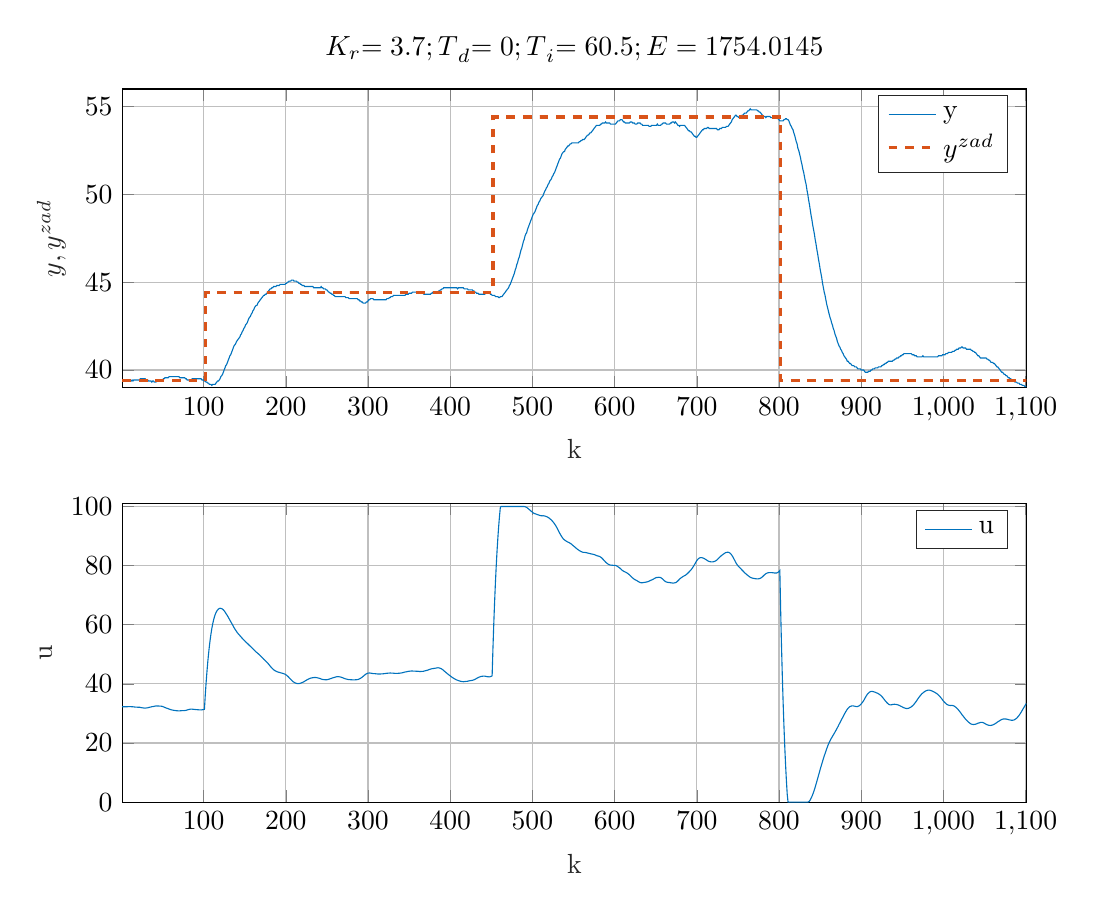
\begin{tikzpicture}

\begin{axis}[%
width=4.521in,
height=1.493in,
at={(0.758in,2.554in)},
scale only axis,
xmin=1,
xmax=1101,
xlabel style={font=\color{white!15!black}},
xlabel={k},
ymin=39,
ymax=56,
ylabel style={font=\color{white!15!black}},
ylabel={$\text{y, y}^{\text{zad}}$},
axis background/.style={fill=white},
title style={font=\bfseries},
title={$\text{K}_\text{r}\text{=3.7; T}_\text{d}\text{=0; T}_\text{i}\text{=60.5; E=1754.0145}$},
xmajorgrids,
ymajorgrids,
legend style={legend cell align=left, align=left, draw=white!15!black}
]
\addplot [color=mycolor1]
  table[row sep=crcr]{%
1	39.37\\
2	39.37\\
3	39.37\\
4	39.37\\
5	39.37\\
6	39.37\\
7	39.37\\
8	39.37\\
9	39.37\\
10	39.37\\
11	39.37\\
12	39.37\\
13	39.43\\
14	39.37\\
15	39.43\\
16	39.43\\
17	39.43\\
18	39.43\\
19	39.43\\
20	39.43\\
21	39.43\\
22	39.43\\
23	39.5\\
24	39.5\\
25	39.5\\
26	39.5\\
27	39.5\\
28	39.5\\
29	39.5\\
30	39.43\\
31	39.43\\
32	39.43\\
33	39.37\\
34	39.37\\
35	39.37\\
36	39.37\\
37	39.31\\
38	39.37\\
39	39.37\\
40	39.31\\
41	39.31\\
42	39.31\\
43	39.37\\
44	39.37\\
45	39.37\\
46	39.37\\
47	39.37\\
48	39.37\\
49	39.43\\
50	39.43\\
51	39.5\\
52	39.5\\
53	39.56\\
54	39.56\\
55	39.56\\
56	39.56\\
57	39.56\\
58	39.62\\
59	39.62\\
60	39.62\\
61	39.62\\
62	39.62\\
63	39.62\\
64	39.62\\
65	39.62\\
66	39.62\\
67	39.62\\
68	39.62\\
69	39.62\\
70	39.62\\
71	39.56\\
72	39.56\\
73	39.56\\
74	39.56\\
75	39.56\\
76	39.56\\
77	39.56\\
78	39.5\\
79	39.5\\
80	39.43\\
81	39.43\\
82	39.43\\
83	39.43\\
84	39.43\\
85	39.43\\
86	39.5\\
87	39.5\\
88	39.5\\
89	39.5\\
90	39.5\\
91	39.5\\
92	39.5\\
93	39.5\\
94	39.5\\
95	39.5\\
96	39.5\\
97	39.5\\
98	39.43\\
99	39.43\\
100	39.43\\
101	39.37\\
102	39.37\\
103	39.31\\
104	39.31\\
105	39.25\\
106	39.25\\
107	39.18\\
108	39.18\\
109	39.18\\
110	39.12\\
111	39.18\\
112	39.18\\
113	39.18\\
114	39.18\\
115	39.25\\
116	39.31\\
117	39.37\\
118	39.37\\
119	39.43\\
120	39.5\\
121	39.62\\
122	39.68\\
123	39.75\\
124	39.87\\
125	40\\
126	40.12\\
127	40.25\\
128	40.31\\
129	40.43\\
130	40.56\\
131	40.68\\
132	40.81\\
133	40.87\\
134	41\\
135	41.12\\
136	41.25\\
137	41.37\\
138	41.43\\
139	41.5\\
140	41.62\\
141	41.68\\
142	41.75\\
143	41.81\\
144	41.87\\
145	42\\
146	42.06\\
147	42.18\\
148	42.25\\
149	42.37\\
150	42.43\\
151	42.56\\
152	42.62\\
153	42.68\\
154	42.81\\
155	42.93\\
156	43\\
157	43.06\\
158	43.18\\
159	43.25\\
160	43.37\\
161	43.43\\
162	43.56\\
163	43.62\\
164	43.68\\
165	43.68\\
166	43.81\\
167	43.87\\
168	43.93\\
169	44\\
170	44.06\\
171	44.12\\
172	44.18\\
173	44.25\\
174	44.25\\
175	44.31\\
176	44.31\\
177	44.37\\
178	44.43\\
179	44.5\\
180	44.56\\
181	44.62\\
182	44.62\\
183	44.68\\
184	44.68\\
185	44.75\\
186	44.75\\
187	44.75\\
188	44.75\\
189	44.81\\
190	44.81\\
191	44.81\\
192	44.81\\
193	44.87\\
194	44.87\\
195	44.87\\
196	44.87\\
197	44.87\\
198	44.87\\
199	44.87\\
200	44.93\\
201	44.93\\
202	45\\
203	45\\
204	45.06\\
205	45.06\\
206	45.06\\
207	45.12\\
208	45.12\\
209	45.12\\
210	45.06\\
211	45.06\\
212	45.06\\
213	45.06\\
214	45\\
215	45\\
216	44.93\\
217	44.93\\
218	44.87\\
219	44.87\\
220	44.81\\
221	44.81\\
222	44.81\\
223	44.75\\
224	44.75\\
225	44.75\\
226	44.75\\
227	44.75\\
228	44.75\\
229	44.75\\
230	44.75\\
231	44.75\\
232	44.75\\
233	44.75\\
234	44.68\\
235	44.68\\
236	44.68\\
237	44.68\\
238	44.68\\
239	44.68\\
240	44.68\\
241	44.68\\
242	44.68\\
243	44.75\\
244	44.68\\
245	44.68\\
246	44.62\\
247	44.62\\
248	44.62\\
249	44.56\\
250	44.56\\
251	44.5\\
252	44.43\\
253	44.43\\
254	44.37\\
255	44.37\\
256	44.31\\
257	44.31\\
258	44.25\\
259	44.25\\
260	44.18\\
261	44.18\\
262	44.18\\
263	44.18\\
264	44.18\\
265	44.18\\
266	44.18\\
267	44.18\\
268	44.18\\
269	44.18\\
270	44.18\\
271	44.18\\
272	44.18\\
273	44.12\\
274	44.12\\
275	44.12\\
276	44.12\\
277	44.06\\
278	44.06\\
279	44.06\\
280	44.06\\
281	44.06\\
282	44.06\\
283	44.06\\
284	44.06\\
285	44.06\\
286	44.06\\
287	44.06\\
288	44\\
289	44\\
290	43.93\\
291	43.93\\
292	43.87\\
293	43.87\\
294	43.81\\
295	43.81\\
296	43.81\\
297	43.81\\
298	43.87\\
299	43.87\\
300	43.93\\
301	44\\
302	44\\
303	44.06\\
304	44.06\\
305	44.06\\
306	44.06\\
307	44\\
308	44\\
309	44\\
310	44\\
311	44\\
312	44\\
313	44\\
314	44\\
315	44\\
316	44\\
317	44\\
318	44\\
319	44\\
320	44\\
321	44\\
322	44\\
323	44.06\\
324	44.06\\
325	44.06\\
326	44.12\\
327	44.12\\
328	44.18\\
329	44.18\\
330	44.18\\
331	44.25\\
332	44.25\\
333	44.25\\
334	44.25\\
335	44.25\\
336	44.25\\
337	44.25\\
338	44.25\\
339	44.25\\
340	44.25\\
341	44.25\\
342	44.25\\
343	44.25\\
344	44.25\\
345	44.25\\
346	44.31\\
347	44.31\\
348	44.31\\
349	44.31\\
350	44.37\\
351	44.37\\
352	44.37\\
353	44.37\\
354	44.43\\
355	44.43\\
356	44.43\\
357	44.43\\
358	44.43\\
359	44.43\\
360	44.43\\
361	44.37\\
362	44.43\\
363	44.43\\
364	44.37\\
365	44.37\\
366	44.37\\
367	44.37\\
368	44.31\\
369	44.31\\
370	44.31\\
371	44.31\\
372	44.31\\
373	44.31\\
374	44.31\\
375	44.31\\
376	44.31\\
377	44.37\\
378	44.37\\
379	44.43\\
380	44.43\\
381	44.43\\
382	44.43\\
383	44.43\\
384	44.43\\
385	44.43\\
386	44.5\\
387	44.5\\
388	44.56\\
389	44.56\\
390	44.62\\
391	44.62\\
392	44.68\\
393	44.68\\
394	44.68\\
395	44.68\\
396	44.68\\
397	44.68\\
398	44.68\\
399	44.68\\
400	44.68\\
401	44.68\\
402	44.68\\
403	44.68\\
404	44.68\\
405	44.68\\
406	44.68\\
407	44.68\\
408	44.68\\
409	44.62\\
410	44.68\\
411	44.68\\
412	44.68\\
413	44.68\\
414	44.68\\
415	44.68\\
416	44.68\\
417	44.62\\
418	44.62\\
419	44.62\\
420	44.62\\
421	44.62\\
422	44.56\\
423	44.56\\
424	44.56\\
425	44.56\\
426	44.56\\
427	44.56\\
428	44.5\\
429	44.5\\
430	44.43\\
431	44.43\\
432	44.37\\
433	44.37\\
434	44.37\\
435	44.31\\
436	44.31\\
437	44.31\\
438	44.31\\
439	44.31\\
440	44.31\\
441	44.31\\
442	44.31\\
443	44.37\\
444	44.37\\
445	44.37\\
446	44.37\\
447	44.37\\
448	44.37\\
449	44.31\\
450	44.31\\
451	44.25\\
452	44.25\\
453	44.25\\
454	44.25\\
455	44.18\\
456	44.18\\
457	44.18\\
458	44.18\\
459	44.12\\
460	44.12\\
461	44.18\\
462	44.18\\
463	44.18\\
464	44.25\\
465	44.31\\
466	44.37\\
467	44.43\\
468	44.5\\
469	44.56\\
470	44.62\\
471	44.68\\
472	44.81\\
473	44.87\\
474	45\\
475	45.12\\
476	45.25\\
477	45.37\\
478	45.5\\
479	45.68\\
480	45.81\\
481	46\\
482	46.12\\
483	46.31\\
484	46.43\\
485	46.62\\
486	46.81\\
487	46.93\\
488	47.12\\
489	47.31\\
490	47.43\\
491	47.62\\
492	47.75\\
493	47.81\\
494	48\\
495	48.12\\
496	48.25\\
497	48.37\\
498	48.5\\
499	48.62\\
500	48.75\\
501	48.87\\
502	48.93\\
503	49\\
504	49.12\\
505	49.25\\
506	49.37\\
507	49.43\\
508	49.56\\
509	49.62\\
510	49.75\\
511	49.81\\
512	49.87\\
513	49.93\\
514	50.06\\
515	50.18\\
516	50.25\\
517	50.37\\
518	50.43\\
519	50.56\\
520	50.62\\
521	50.75\\
522	50.81\\
523	50.87\\
524	51\\
525	51.06\\
526	51.18\\
527	51.25\\
528	51.37\\
529	51.5\\
530	51.62\\
531	51.75\\
532	51.87\\
533	52\\
534	52.06\\
535	52.18\\
536	52.31\\
537	52.37\\
538	52.43\\
539	52.43\\
540	52.56\\
541	52.62\\
542	52.68\\
543	52.75\\
544	52.75\\
545	52.81\\
546	52.87\\
547	52.87\\
548	52.93\\
549	52.93\\
550	52.93\\
551	52.93\\
552	52.93\\
553	52.93\\
554	52.93\\
555	52.93\\
556	52.93\\
557	53\\
558	53\\
559	53.06\\
560	53.06\\
561	53.12\\
562	53.12\\
563	53.12\\
564	53.18\\
565	53.25\\
566	53.31\\
567	53.37\\
568	53.37\\
569	53.43\\
570	53.5\\
571	53.5\\
572	53.56\\
573	53.62\\
574	53.68\\
575	53.75\\
576	53.81\\
577	53.87\\
578	53.93\\
579	53.93\\
580	53.93\\
581	53.93\\
582	53.93\\
583	54\\
584	54\\
585	54.06\\
586	54.06\\
587	54.06\\
588	54.06\\
589	54.12\\
590	54.06\\
591	54.06\\
592	54.06\\
593	54.06\\
594	54.06\\
595	54\\
596	54\\
597	54\\
598	54\\
599	54\\
600	54\\
601	54\\
602	54.06\\
603	54.12\\
604	54.18\\
605	54.18\\
606	54.18\\
607	54.25\\
608	54.25\\
609	54.25\\
610	54.18\\
611	54.12\\
612	54.12\\
613	54.06\\
614	54.06\\
615	54.06\\
616	54.06\\
617	54.06\\
618	54.06\\
619	54.12\\
620	54.12\\
621	54.12\\
622	54.06\\
623	54.06\\
624	54.06\\
625	54\\
626	54\\
627	54\\
628	54.06\\
629	54.06\\
630	54.06\\
631	54.06\\
632	54\\
633	54\\
634	53.93\\
635	53.93\\
636	53.93\\
637	53.93\\
638	53.93\\
639	53.93\\
640	53.93\\
641	53.93\\
642	53.87\\
643	53.87\\
644	53.87\\
645	53.93\\
646	53.93\\
647	53.93\\
648	53.93\\
649	53.93\\
650	53.93\\
651	53.93\\
652	54\\
653	53.93\\
654	53.93\\
655	53.93\\
656	53.93\\
657	54\\
658	54\\
659	54.06\\
660	54.06\\
661	54.06\\
662	54.06\\
663	54\\
664	54\\
665	54\\
666	54\\
667	54\\
668	54.06\\
669	54.06\\
670	54.12\\
671	54.12\\
672	54.12\\
673	54.06\\
674	54.12\\
675	54.06\\
676	54\\
677	53.93\\
678	53.93\\
679	53.87\\
680	53.93\\
681	53.93\\
682	53.93\\
683	53.93\\
684	53.93\\
685	53.93\\
686	53.87\\
687	53.81\\
688	53.75\\
689	53.68\\
690	53.62\\
691	53.62\\
692	53.56\\
693	53.56\\
694	53.5\\
695	53.43\\
696	53.37\\
697	53.31\\
698	53.31\\
699	53.25\\
700	53.25\\
701	53.31\\
702	53.37\\
703	53.43\\
704	53.5\\
705	53.56\\
706	53.62\\
707	53.68\\
708	53.68\\
709	53.75\\
710	53.75\\
711	53.75\\
712	53.75\\
713	53.81\\
714	53.81\\
715	53.75\\
716	53.75\\
717	53.75\\
718	53.75\\
719	53.75\\
720	53.75\\
721	53.75\\
722	53.75\\
723	53.75\\
724	53.75\\
725	53.68\\
726	53.68\\
727	53.68\\
728	53.75\\
729	53.75\\
730	53.75\\
731	53.81\\
732	53.81\\
733	53.81\\
734	53.81\\
735	53.81\\
736	53.87\\
737	53.87\\
738	53.87\\
739	53.93\\
740	54\\
741	54.06\\
742	54.12\\
743	54.25\\
744	54.31\\
745	54.37\\
746	54.43\\
747	54.5\\
748	54.5\\
749	54.43\\
750	54.43\\
751	54.37\\
752	54.37\\
753	54.43\\
754	54.43\\
755	54.5\\
756	54.5\\
757	54.56\\
758	54.62\\
759	54.62\\
760	54.62\\
761	54.68\\
762	54.75\\
763	54.75\\
764	54.81\\
765	54.87\\
766	54.81\\
767	54.81\\
768	54.81\\
769	54.81\\
770	54.81\\
771	54.81\\
772	54.81\\
773	54.81\\
774	54.75\\
775	54.75\\
776	54.68\\
777	54.68\\
778	54.62\\
779	54.56\\
780	54.5\\
781	54.43\\
782	54.43\\
783	54.43\\
784	54.37\\
785	54.43\\
786	54.43\\
787	54.43\\
788	54.43\\
789	54.43\\
790	54.37\\
791	54.37\\
792	54.37\\
793	54.37\\
794	54.37\\
795	54.37\\
796	54.37\\
797	54.37\\
798	54.31\\
799	54.31\\
800	54.25\\
801	54.18\\
802	54.18\\
803	54.18\\
804	54.18\\
805	54.18\\
806	54.25\\
807	54.25\\
808	54.31\\
809	54.31\\
810	54.25\\
811	54.25\\
812	54.18\\
813	54.06\\
814	53.93\\
815	53.87\\
816	53.75\\
817	53.68\\
818	53.5\\
819	53.37\\
820	53.18\\
821	53\\
822	52.87\\
823	52.62\\
824	52.5\\
825	52.31\\
826	52.12\\
827	51.87\\
828	51.68\\
829	51.43\\
830	51.25\\
831	51\\
832	50.75\\
833	50.56\\
834	50.25\\
835	50\\
836	49.68\\
837	49.43\\
838	49.12\\
839	48.81\\
840	48.56\\
841	48.25\\
842	48\\
843	47.75\\
844	47.43\\
845	47.18\\
846	46.87\\
847	46.62\\
848	46.31\\
849	46.06\\
850	45.75\\
851	45.5\\
852	45.25\\
853	44.93\\
854	44.68\\
855	44.43\\
856	44.25\\
857	44\\
858	43.75\\
859	43.56\\
860	43.37\\
861	43.18\\
862	43\\
863	42.87\\
864	42.68\\
865	42.56\\
866	42.37\\
867	42.25\\
868	42.06\\
869	41.93\\
870	41.81\\
871	41.62\\
872	41.5\\
873	41.37\\
874	41.31\\
875	41.18\\
876	41.12\\
877	41\\
878	40.93\\
879	40.81\\
880	40.75\\
881	40.68\\
882	40.62\\
883	40.5\\
884	40.5\\
885	40.43\\
886	40.37\\
887	40.37\\
888	40.31\\
889	40.25\\
890	40.25\\
891	40.25\\
892	40.18\\
893	40.18\\
894	40.18\\
895	40.12\\
896	40.06\\
897	40.06\\
898	40.06\\
899	40.06\\
900	40\\
901	40\\
902	40\\
903	40\\
904	39.93\\
905	39.87\\
906	39.87\\
907	39.87\\
908	39.87\\
909	39.93\\
910	39.93\\
911	39.93\\
912	40\\
913	40\\
914	40.06\\
915	40.06\\
916	40.06\\
917	40.12\\
918	40.12\\
919	40.12\\
920	40.12\\
921	40.18\\
922	40.18\\
923	40.18\\
924	40.18\\
925	40.25\\
926	40.25\\
927	40.31\\
928	40.31\\
929	40.37\\
930	40.37\\
931	40.43\\
932	40.43\\
933	40.5\\
934	40.5\\
935	40.5\\
936	40.5\\
937	40.5\\
938	40.5\\
939	40.56\\
940	40.56\\
941	40.62\\
942	40.62\\
943	40.68\\
944	40.68\\
945	40.68\\
946	40.75\\
947	40.75\\
948	40.81\\
949	40.81\\
950	40.87\\
951	40.87\\
952	40.93\\
953	40.93\\
954	40.93\\
955	40.93\\
956	40.93\\
957	40.93\\
958	40.93\\
959	40.93\\
960	40.93\\
961	40.93\\
962	40.87\\
963	40.87\\
964	40.87\\
965	40.81\\
966	40.81\\
967	40.81\\
968	40.75\\
969	40.75\\
970	40.75\\
971	40.75\\
972	40.75\\
973	40.75\\
974	40.75\\
975	40.81\\
976	40.75\\
977	40.75\\
978	40.75\\
979	40.75\\
980	40.75\\
981	40.75\\
982	40.75\\
983	40.75\\
984	40.75\\
985	40.75\\
986	40.75\\
987	40.75\\
988	40.75\\
989	40.75\\
990	40.75\\
991	40.75\\
992	40.75\\
993	40.75\\
994	40.81\\
995	40.81\\
996	40.81\\
997	40.81\\
998	40.81\\
999	40.87\\
1000	40.87\\
1001	40.87\\
1002	40.87\\
1003	40.93\\
1004	40.93\\
1005	40.93\\
1006	41\\
1007	41\\
1008	41\\
1009	41\\
1010	41\\
1011	41.06\\
1012	41.06\\
1013	41.06\\
1014	41.12\\
1015	41.12\\
1016	41.18\\
1017	41.18\\
1018	41.18\\
1019	41.25\\
1020	41.25\\
1021	41.25\\
1022	41.31\\
1023	41.31\\
1024	41.25\\
1025	41.25\\
1026	41.25\\
1027	41.25\\
1028	41.18\\
1029	41.18\\
1030	41.18\\
1031	41.18\\
1032	41.18\\
1033	41.18\\
1034	41.12\\
1035	41.12\\
1036	41.06\\
1037	41.06\\
1038	41\\
1039	41\\
1040	40.93\\
1041	40.87\\
1042	40.81\\
1043	40.81\\
1044	40.75\\
1045	40.68\\
1046	40.68\\
1047	40.68\\
1048	40.68\\
1049	40.68\\
1050	40.68\\
1051	40.68\\
1052	40.68\\
1053	40.62\\
1054	40.62\\
1055	40.56\\
1056	40.56\\
1057	40.5\\
1058	40.43\\
1059	40.43\\
1060	40.43\\
1061	40.37\\
1062	40.37\\
1063	40.31\\
1064	40.25\\
1065	40.18\\
1066	40.18\\
1067	40.12\\
1068	40.06\\
1069	40\\
1070	39.93\\
1071	39.87\\
1072	39.87\\
1073	39.81\\
1074	39.75\\
1075	39.75\\
1076	39.68\\
1077	39.68\\
1078	39.62\\
1079	39.56\\
1080	39.56\\
1081	39.5\\
1082	39.5\\
1083	39.43\\
1084	39.43\\
1085	39.37\\
1086	39.37\\
1087	39.31\\
1088	39.31\\
1089	39.31\\
1090	39.25\\
1091	39.25\\
1092	39.25\\
1093	39.18\\
1094	39.18\\
1095	39.18\\
1096	39.12\\
1097	39.12\\
1098	39.12\\
1099	39.06\\
1100	39.06\\
1101	39.06\\
};
\addlegendentry{y}

\addplot[const plot, color=mycolor2, dashed, line width=1.2pt] table[row sep=crcr] {%
1	39.4\\
2	39.4\\
3	39.4\\
4	39.4\\
5	39.4\\
6	39.4\\
7	39.4\\
8	39.4\\
9	39.4\\
10	39.4\\
11	39.4\\
12	39.4\\
13	39.4\\
14	39.4\\
15	39.4\\
16	39.4\\
17	39.4\\
18	39.4\\
19	39.4\\
20	39.4\\
21	39.4\\
22	39.4\\
23	39.4\\
24	39.4\\
25	39.4\\
26	39.4\\
27	39.4\\
28	39.4\\
29	39.4\\
30	39.4\\
31	39.4\\
32	39.4\\
33	39.4\\
34	39.4\\
35	39.4\\
36	39.4\\
37	39.4\\
38	39.4\\
39	39.4\\
40	39.4\\
41	39.4\\
42	39.4\\
43	39.4\\
44	39.4\\
45	39.4\\
46	39.4\\
47	39.4\\
48	39.4\\
49	39.4\\
50	39.4\\
51	39.4\\
52	39.4\\
53	39.4\\
54	39.4\\
55	39.4\\
56	39.4\\
57	39.4\\
58	39.4\\
59	39.4\\
60	39.4\\
61	39.4\\
62	39.4\\
63	39.4\\
64	39.4\\
65	39.4\\
66	39.4\\
67	39.4\\
68	39.4\\
69	39.4\\
70	39.4\\
71	39.4\\
72	39.4\\
73	39.4\\
74	39.4\\
75	39.4\\
76	39.4\\
77	39.4\\
78	39.4\\
79	39.4\\
80	39.4\\
81	39.4\\
82	39.4\\
83	39.4\\
84	39.4\\
85	39.4\\
86	39.4\\
87	39.4\\
88	39.4\\
89	39.4\\
90	39.4\\
91	39.4\\
92	39.4\\
93	39.4\\
94	39.4\\
95	39.4\\
96	39.4\\
97	39.4\\
98	39.4\\
99	39.4\\
100	39.4\\
101	39.4\\
102	44.4\\
103	44.4\\
104	44.4\\
105	44.4\\
106	44.4\\
107	44.4\\
108	44.4\\
109	44.4\\
110	44.4\\
111	44.4\\
112	44.4\\
113	44.4\\
114	44.4\\
115	44.4\\
116	44.4\\
117	44.4\\
118	44.4\\
119	44.4\\
120	44.4\\
121	44.4\\
122	44.4\\
123	44.4\\
124	44.4\\
125	44.4\\
126	44.4\\
127	44.4\\
128	44.4\\
129	44.4\\
130	44.4\\
131	44.4\\
132	44.4\\
133	44.4\\
134	44.4\\
135	44.4\\
136	44.4\\
137	44.4\\
138	44.4\\
139	44.4\\
140	44.4\\
141	44.4\\
142	44.4\\
143	44.4\\
144	44.4\\
145	44.4\\
146	44.4\\
147	44.4\\
148	44.4\\
149	44.4\\
150	44.4\\
151	44.4\\
152	44.4\\
153	44.4\\
154	44.4\\
155	44.4\\
156	44.4\\
157	44.4\\
158	44.4\\
159	44.4\\
160	44.4\\
161	44.4\\
162	44.4\\
163	44.4\\
164	44.4\\
165	44.4\\
166	44.4\\
167	44.4\\
168	44.4\\
169	44.4\\
170	44.4\\
171	44.4\\
172	44.4\\
173	44.4\\
174	44.4\\
175	44.4\\
176	44.4\\
177	44.4\\
178	44.4\\
179	44.4\\
180	44.4\\
181	44.4\\
182	44.4\\
183	44.4\\
184	44.4\\
185	44.4\\
186	44.4\\
187	44.4\\
188	44.4\\
189	44.4\\
190	44.4\\
191	44.4\\
192	44.4\\
193	44.4\\
194	44.4\\
195	44.4\\
196	44.4\\
197	44.4\\
198	44.4\\
199	44.4\\
200	44.4\\
201	44.4\\
202	44.4\\
203	44.4\\
204	44.4\\
205	44.4\\
206	44.4\\
207	44.4\\
208	44.4\\
209	44.4\\
210	44.4\\
211	44.4\\
212	44.4\\
213	44.4\\
214	44.4\\
215	44.4\\
216	44.4\\
217	44.4\\
218	44.4\\
219	44.4\\
220	44.4\\
221	44.4\\
222	44.4\\
223	44.4\\
224	44.4\\
225	44.4\\
226	44.4\\
227	44.4\\
228	44.4\\
229	44.4\\
230	44.4\\
231	44.4\\
232	44.4\\
233	44.4\\
234	44.4\\
235	44.4\\
236	44.4\\
237	44.4\\
238	44.4\\
239	44.4\\
240	44.4\\
241	44.4\\
242	44.4\\
243	44.4\\
244	44.4\\
245	44.4\\
246	44.4\\
247	44.4\\
248	44.4\\
249	44.4\\
250	44.4\\
251	44.4\\
252	44.4\\
253	44.4\\
254	44.4\\
255	44.4\\
256	44.4\\
257	44.4\\
258	44.4\\
259	44.4\\
260	44.4\\
261	44.4\\
262	44.4\\
263	44.4\\
264	44.4\\
265	44.4\\
266	44.4\\
267	44.4\\
268	44.4\\
269	44.4\\
270	44.4\\
271	44.4\\
272	44.4\\
273	44.4\\
274	44.4\\
275	44.4\\
276	44.4\\
277	44.4\\
278	44.4\\
279	44.4\\
280	44.4\\
281	44.4\\
282	44.4\\
283	44.4\\
284	44.4\\
285	44.4\\
286	44.4\\
287	44.4\\
288	44.4\\
289	44.4\\
290	44.4\\
291	44.4\\
292	44.4\\
293	44.4\\
294	44.4\\
295	44.4\\
296	44.4\\
297	44.4\\
298	44.4\\
299	44.4\\
300	44.4\\
301	44.4\\
302	44.4\\
303	44.4\\
304	44.4\\
305	44.4\\
306	44.4\\
307	44.4\\
308	44.4\\
309	44.4\\
310	44.4\\
311	44.4\\
312	44.4\\
313	44.4\\
314	44.4\\
315	44.4\\
316	44.4\\
317	44.4\\
318	44.4\\
319	44.4\\
320	44.4\\
321	44.4\\
322	44.4\\
323	44.4\\
324	44.4\\
325	44.4\\
326	44.4\\
327	44.4\\
328	44.4\\
329	44.4\\
330	44.4\\
331	44.4\\
332	44.4\\
333	44.4\\
334	44.4\\
335	44.4\\
336	44.4\\
337	44.4\\
338	44.4\\
339	44.4\\
340	44.4\\
341	44.4\\
342	44.4\\
343	44.4\\
344	44.4\\
345	44.4\\
346	44.4\\
347	44.4\\
348	44.4\\
349	44.4\\
350	44.4\\
351	44.4\\
352	44.4\\
353	44.4\\
354	44.4\\
355	44.4\\
356	44.4\\
357	44.4\\
358	44.4\\
359	44.4\\
360	44.4\\
361	44.4\\
362	44.4\\
363	44.4\\
364	44.4\\
365	44.4\\
366	44.4\\
367	44.4\\
368	44.4\\
369	44.4\\
370	44.4\\
371	44.4\\
372	44.4\\
373	44.4\\
374	44.4\\
375	44.4\\
376	44.4\\
377	44.4\\
378	44.4\\
379	44.4\\
380	44.4\\
381	44.4\\
382	44.4\\
383	44.4\\
384	44.4\\
385	44.4\\
386	44.4\\
387	44.4\\
388	44.4\\
389	44.4\\
390	44.4\\
391	44.4\\
392	44.4\\
393	44.4\\
394	44.4\\
395	44.4\\
396	44.4\\
397	44.4\\
398	44.4\\
399	44.4\\
400	44.4\\
401	44.4\\
402	44.4\\
403	44.4\\
404	44.4\\
405	44.4\\
406	44.4\\
407	44.4\\
408	44.4\\
409	44.4\\
410	44.4\\
411	44.4\\
412	44.4\\
413	44.4\\
414	44.4\\
415	44.4\\
416	44.4\\
417	44.4\\
418	44.4\\
419	44.4\\
420	44.4\\
421	44.4\\
422	44.4\\
423	44.4\\
424	44.4\\
425	44.4\\
426	44.4\\
427	44.4\\
428	44.4\\
429	44.4\\
430	44.4\\
431	44.4\\
432	44.4\\
433	44.4\\
434	44.4\\
435	44.4\\
436	44.4\\
437	44.4\\
438	44.4\\
439	44.4\\
440	44.4\\
441	44.4\\
442	44.4\\
443	44.4\\
444	44.4\\
445	44.4\\
446	44.4\\
447	44.4\\
448	44.4\\
449	44.4\\
450	44.4\\
451	44.4\\
452	54.4\\
453	54.4\\
454	54.4\\
455	54.4\\
456	54.4\\
457	54.4\\
458	54.4\\
459	54.4\\
460	54.4\\
461	54.4\\
462	54.4\\
463	54.4\\
464	54.4\\
465	54.4\\
466	54.4\\
467	54.4\\
468	54.4\\
469	54.4\\
470	54.4\\
471	54.4\\
472	54.4\\
473	54.4\\
474	54.4\\
475	54.4\\
476	54.4\\
477	54.4\\
478	54.4\\
479	54.4\\
480	54.4\\
481	54.4\\
482	54.4\\
483	54.4\\
484	54.4\\
485	54.4\\
486	54.4\\
487	54.4\\
488	54.4\\
489	54.4\\
490	54.4\\
491	54.4\\
492	54.4\\
493	54.4\\
494	54.4\\
495	54.4\\
496	54.4\\
497	54.4\\
498	54.4\\
499	54.4\\
500	54.4\\
501	54.4\\
502	54.4\\
503	54.4\\
504	54.4\\
505	54.4\\
506	54.4\\
507	54.4\\
508	54.4\\
509	54.4\\
510	54.4\\
511	54.4\\
512	54.4\\
513	54.4\\
514	54.4\\
515	54.4\\
516	54.4\\
517	54.4\\
518	54.4\\
519	54.4\\
520	54.4\\
521	54.4\\
522	54.4\\
523	54.4\\
524	54.4\\
525	54.4\\
526	54.4\\
527	54.4\\
528	54.4\\
529	54.4\\
530	54.4\\
531	54.4\\
532	54.4\\
533	54.4\\
534	54.4\\
535	54.4\\
536	54.4\\
537	54.4\\
538	54.4\\
539	54.4\\
540	54.4\\
541	54.4\\
542	54.4\\
543	54.4\\
544	54.4\\
545	54.4\\
546	54.4\\
547	54.4\\
548	54.4\\
549	54.4\\
550	54.4\\
551	54.4\\
552	54.4\\
553	54.4\\
554	54.4\\
555	54.4\\
556	54.4\\
557	54.4\\
558	54.4\\
559	54.4\\
560	54.4\\
561	54.4\\
562	54.4\\
563	54.4\\
564	54.4\\
565	54.4\\
566	54.4\\
567	54.4\\
568	54.4\\
569	54.4\\
570	54.4\\
571	54.4\\
572	54.4\\
573	54.4\\
574	54.4\\
575	54.4\\
576	54.4\\
577	54.4\\
578	54.4\\
579	54.4\\
580	54.4\\
581	54.4\\
582	54.4\\
583	54.4\\
584	54.4\\
585	54.4\\
586	54.4\\
587	54.4\\
588	54.4\\
589	54.4\\
590	54.4\\
591	54.4\\
592	54.4\\
593	54.4\\
594	54.4\\
595	54.4\\
596	54.4\\
597	54.4\\
598	54.4\\
599	54.4\\
600	54.4\\
601	54.4\\
602	54.4\\
603	54.4\\
604	54.4\\
605	54.4\\
606	54.4\\
607	54.4\\
608	54.4\\
609	54.4\\
610	54.4\\
611	54.4\\
612	54.4\\
613	54.4\\
614	54.4\\
615	54.4\\
616	54.4\\
617	54.4\\
618	54.4\\
619	54.4\\
620	54.4\\
621	54.4\\
622	54.4\\
623	54.4\\
624	54.4\\
625	54.4\\
626	54.4\\
627	54.4\\
628	54.4\\
629	54.4\\
630	54.4\\
631	54.4\\
632	54.4\\
633	54.4\\
634	54.4\\
635	54.4\\
636	54.4\\
637	54.4\\
638	54.4\\
639	54.4\\
640	54.4\\
641	54.4\\
642	54.4\\
643	54.4\\
644	54.4\\
645	54.4\\
646	54.4\\
647	54.4\\
648	54.4\\
649	54.4\\
650	54.4\\
651	54.4\\
652	54.4\\
653	54.4\\
654	54.4\\
655	54.4\\
656	54.4\\
657	54.4\\
658	54.4\\
659	54.4\\
660	54.4\\
661	54.4\\
662	54.4\\
663	54.4\\
664	54.4\\
665	54.4\\
666	54.4\\
667	54.4\\
668	54.4\\
669	54.4\\
670	54.4\\
671	54.4\\
672	54.4\\
673	54.4\\
674	54.4\\
675	54.4\\
676	54.4\\
677	54.4\\
678	54.4\\
679	54.4\\
680	54.4\\
681	54.4\\
682	54.4\\
683	54.4\\
684	54.4\\
685	54.4\\
686	54.4\\
687	54.4\\
688	54.4\\
689	54.4\\
690	54.4\\
691	54.4\\
692	54.4\\
693	54.4\\
694	54.4\\
695	54.4\\
696	54.4\\
697	54.4\\
698	54.4\\
699	54.4\\
700	54.4\\
701	54.4\\
702	54.4\\
703	54.4\\
704	54.4\\
705	54.4\\
706	54.4\\
707	54.4\\
708	54.4\\
709	54.4\\
710	54.4\\
711	54.4\\
712	54.4\\
713	54.4\\
714	54.4\\
715	54.4\\
716	54.4\\
717	54.4\\
718	54.4\\
719	54.4\\
720	54.4\\
721	54.4\\
722	54.4\\
723	54.4\\
724	54.4\\
725	54.4\\
726	54.4\\
727	54.4\\
728	54.4\\
729	54.4\\
730	54.4\\
731	54.4\\
732	54.4\\
733	54.4\\
734	54.4\\
735	54.4\\
736	54.4\\
737	54.4\\
738	54.4\\
739	54.4\\
740	54.4\\
741	54.4\\
742	54.4\\
743	54.4\\
744	54.4\\
745	54.4\\
746	54.4\\
747	54.4\\
748	54.4\\
749	54.4\\
750	54.4\\
751	54.4\\
752	54.4\\
753	54.4\\
754	54.4\\
755	54.4\\
756	54.4\\
757	54.4\\
758	54.4\\
759	54.4\\
760	54.4\\
761	54.4\\
762	54.4\\
763	54.4\\
764	54.4\\
765	54.4\\
766	54.4\\
767	54.4\\
768	54.4\\
769	54.4\\
770	54.4\\
771	54.4\\
772	54.4\\
773	54.4\\
774	54.4\\
775	54.4\\
776	54.4\\
777	54.4\\
778	54.4\\
779	54.4\\
780	54.4\\
781	54.4\\
782	54.4\\
783	54.4\\
784	54.4\\
785	54.4\\
786	54.4\\
787	54.4\\
788	54.4\\
789	54.4\\
790	54.4\\
791	54.4\\
792	54.4\\
793	54.4\\
794	54.4\\
795	54.4\\
796	54.4\\
797	54.4\\
798	54.4\\
799	54.4\\
800	54.4\\
801	54.4\\
802	39.4\\
803	39.4\\
804	39.4\\
805	39.4\\
806	39.4\\
807	39.4\\
808	39.4\\
809	39.4\\
810	39.4\\
811	39.4\\
812	39.4\\
813	39.4\\
814	39.4\\
815	39.4\\
816	39.4\\
817	39.4\\
818	39.4\\
819	39.4\\
820	39.4\\
821	39.4\\
822	39.4\\
823	39.4\\
824	39.4\\
825	39.4\\
826	39.4\\
827	39.4\\
828	39.4\\
829	39.4\\
830	39.4\\
831	39.4\\
832	39.4\\
833	39.4\\
834	39.4\\
835	39.4\\
836	39.4\\
837	39.4\\
838	39.4\\
839	39.4\\
840	39.4\\
841	39.4\\
842	39.4\\
843	39.4\\
844	39.4\\
845	39.4\\
846	39.4\\
847	39.4\\
848	39.4\\
849	39.4\\
850	39.4\\
851	39.4\\
852	39.4\\
853	39.4\\
854	39.4\\
855	39.4\\
856	39.4\\
857	39.4\\
858	39.4\\
859	39.4\\
860	39.4\\
861	39.4\\
862	39.4\\
863	39.4\\
864	39.4\\
865	39.4\\
866	39.4\\
867	39.4\\
868	39.4\\
869	39.4\\
870	39.4\\
871	39.4\\
872	39.4\\
873	39.4\\
874	39.4\\
875	39.4\\
876	39.4\\
877	39.4\\
878	39.4\\
879	39.4\\
880	39.4\\
881	39.4\\
882	39.4\\
883	39.4\\
884	39.4\\
885	39.4\\
886	39.4\\
887	39.4\\
888	39.4\\
889	39.4\\
890	39.4\\
891	39.4\\
892	39.4\\
893	39.4\\
894	39.4\\
895	39.4\\
896	39.4\\
897	39.4\\
898	39.4\\
899	39.4\\
900	39.4\\
901	39.4\\
902	39.4\\
903	39.4\\
904	39.4\\
905	39.4\\
906	39.4\\
907	39.4\\
908	39.4\\
909	39.4\\
910	39.4\\
911	39.4\\
912	39.4\\
913	39.4\\
914	39.4\\
915	39.4\\
916	39.4\\
917	39.4\\
918	39.4\\
919	39.4\\
920	39.4\\
921	39.4\\
922	39.4\\
923	39.4\\
924	39.4\\
925	39.4\\
926	39.4\\
927	39.4\\
928	39.4\\
929	39.4\\
930	39.4\\
931	39.4\\
932	39.4\\
933	39.4\\
934	39.4\\
935	39.4\\
936	39.4\\
937	39.4\\
938	39.4\\
939	39.4\\
940	39.4\\
941	39.4\\
942	39.4\\
943	39.4\\
944	39.4\\
945	39.4\\
946	39.4\\
947	39.4\\
948	39.4\\
949	39.4\\
950	39.4\\
951	39.4\\
952	39.4\\
953	39.4\\
954	39.4\\
955	39.4\\
956	39.4\\
957	39.4\\
958	39.4\\
959	39.4\\
960	39.4\\
961	39.4\\
962	39.4\\
963	39.4\\
964	39.4\\
965	39.4\\
966	39.4\\
967	39.4\\
968	39.4\\
969	39.4\\
970	39.4\\
971	39.4\\
972	39.4\\
973	39.4\\
974	39.4\\
975	39.4\\
976	39.4\\
977	39.4\\
978	39.4\\
979	39.4\\
980	39.4\\
981	39.4\\
982	39.4\\
983	39.4\\
984	39.4\\
985	39.4\\
986	39.4\\
987	39.4\\
988	39.4\\
989	39.4\\
990	39.4\\
991	39.4\\
992	39.4\\
993	39.4\\
994	39.4\\
995	39.4\\
996	39.4\\
997	39.4\\
998	39.4\\
999	39.4\\
1000	39.4\\
1001	39.4\\
1002	39.4\\
1003	39.4\\
1004	39.4\\
1005	39.4\\
1006	39.4\\
1007	39.4\\
1008	39.4\\
1009	39.4\\
1010	39.4\\
1011	39.4\\
1012	39.4\\
1013	39.4\\
1014	39.4\\
1015	39.4\\
1016	39.4\\
1017	39.4\\
1018	39.4\\
1019	39.4\\
1020	39.4\\
1021	39.4\\
1022	39.4\\
1023	39.4\\
1024	39.4\\
1025	39.4\\
1026	39.4\\
1027	39.4\\
1028	39.4\\
1029	39.4\\
1030	39.4\\
1031	39.4\\
1032	39.4\\
1033	39.4\\
1034	39.4\\
1035	39.4\\
1036	39.4\\
1037	39.4\\
1038	39.4\\
1039	39.4\\
1040	39.4\\
1041	39.4\\
1042	39.4\\
1043	39.4\\
1044	39.4\\
1045	39.4\\
1046	39.4\\
1047	39.4\\
1048	39.4\\
1049	39.4\\
1050	39.4\\
1051	39.4\\
1052	39.4\\
1053	39.4\\
1054	39.4\\
1055	39.4\\
1056	39.4\\
1057	39.4\\
1058	39.4\\
1059	39.4\\
1060	39.4\\
1061	39.4\\
1062	39.4\\
1063	39.4\\
1064	39.4\\
1065	39.4\\
1066	39.4\\
1067	39.4\\
1068	39.4\\
1069	39.4\\
1070	39.4\\
1071	39.4\\
1072	39.4\\
1073	39.4\\
1074	39.4\\
1075	39.4\\
1076	39.4\\
1077	39.4\\
1078	39.4\\
1079	39.4\\
1080	39.4\\
1081	39.4\\
1082	39.4\\
1083	39.4\\
1084	39.4\\
1085	39.4\\
1086	39.4\\
1087	39.4\\
1088	39.4\\
1089	39.4\\
1090	39.4\\
1091	39.4\\
1092	39.4\\
1093	39.4\\
1094	39.4\\
1095	39.4\\
1096	39.4\\
1097	39.4\\
1098	39.4\\
1099	39.4\\
1100	39.4\\
1101	39.4\\
};
\addlegendentry{$\text{y}^{\text{zad}}$}

\end{axis}

\begin{axis}[%
width=4.521in,
height=1.493in,
at={(0.758in,0.481in)},
scale only axis,
xmin=1,
xmax=1101,
xlabel style={font=\color{white!15!black}},
xlabel={k},
ymin=0,
ymax=101,
ylabel style={font=\color{white!15!black}},
ylabel={u},
axis background/.style={fill=white},
xmajorgrids,
ymajorgrids,
legend style={legend cell align=left, align=left, draw=white!15!black}
]
\addplot [color=mycolor1]
  table[row sep=crcr]{%
1	32.2533102445048\\
2	32.2603920792043\\
3	32.2668593706072\\
4	32.2726690620953\\
5	32.2773999391396\\
6	32.281139474729\\
7	32.2847071948283\\
8	32.2883448850433\\
9	32.2918673002382\\
10	32.295622899218\\
11	32.2994505816979\\
12	32.3036860152063\\
13	32.2536476057642\\
14	32.2653701837995\\
15	32.2230375582044\\
16	32.1880500275565\\
17	32.1599519049991\\
18	32.1376777819454\\
19	32.1213430785618\\
20	32.1100710056452\\
21	32.102696844241\\
22	32.0986603065934\\
23	32.0337165925026\\
24	31.9783418156705\\
25	31.9310970764176\\
26	31.8910272173794\\
27	31.8571032744574\\
28	31.8281580941836\\
29	31.8032385175931\\
30	31.8456969187004\\
31	31.8838170188314\\
32	31.9173451192961\\
33	32.0012894169119\\
34	32.074787640205\\
35	32.1387565931159\\
36	32.1928689103092\\
37	32.2937522665143\\
38	32.3260369711211\\
39	32.3519446332457\\
40	32.4265866449922\\
41	32.4907968787576\\
42	32.545258289799\\
43	32.5361499289287\\
44	32.5260150673848\\
45	32.5150449228932\\
46	32.5039606199843\\
47	32.4930171328622\\
48	32.4834709400954\\
49	32.4201774006253\\
50	32.3645316321094\\
51	32.252336961879\\
52	32.1540810618212\\
53	32.0136891742238\\
54	31.8909488887093\\
55	31.7842272520871\\
56	31.6924829973118\\
57	31.6139452902887\\
58	31.4926594068626\\
59	31.3875877212127\\
60	31.2972781394419\\
61	31.2196531303858\\
62	31.1528543358487\\
63	31.0960801292589\\
64	31.0468727404434\\
65	31.0035983517549\\
66	30.9661147274889\\
67	30.9329711007864\\
68	30.9035812050913\\
69	30.8769647177973\\
70	30.8525846382633\\
71	30.8845630285756\\
72	30.9120182070826\\
73	30.9341441888656\\
74	30.9513315310093\\
75	30.9639373489096\\
76	30.9725185934215\\
77	30.9776154527579\\
78	31.0337506260277\\
79	31.0806798503916\\
80	31.1824207177199\\
81	31.2682454300888\\
82	31.3404637406767\\
83	31.3996679938617\\
84	31.447876359732\\
85	31.4866220017504\\
86	31.4540578798317\\
87	31.4214443845458\\
88	31.389720909935\\
89	31.3594668930843\\
90	31.330314348506\\
91	31.3035243870349\\
92	31.2791053973057\\
93	31.256606699418\\
94	31.2362400298274\\
95	31.2177286404825\\
96	31.2009245566426\\
97	31.1857745176547\\
98	31.2361377700091\\
99	31.2806028533305\\
100	31.319748788323\\
101	31.4096243626676\\
102	36.0448878712253\\
103	40.2096259770034\\
104	43.8922848226517\\
105	47.1939773230218\\
106	50.0943789417495\\
107	52.6954752545921\\
108	54.9714231149885\\
109	56.9528555493327\\
110	58.7222715897235\\
111	60.1892498605638\\
112	61.4381604400956\\
113	62.5013111724193\\
114	63.3965847471147\\
115	64.0880366452639\\
116	64.6151050584411\\
117	64.9914311098966\\
118	65.2955535975433\\
119	65.48757189714\\
120	65.578992360726\\
121	65.5404343770883\\
122	65.4455023213516\\
123	65.2954358363773\\
124	65.0579147453472\\
125	64.7366424176944\\
126	64.3539549926057\\
127	63.910048185352\\
128	63.4920483561379\\
129	63.0439886970454\\
130	62.5602267331921\\
131	62.0572614444604\\
132	61.5393439836578\\
133	61.0703966845217\\
134	60.5826904467763\\
135	60.0872014716575\\
136	59.5756097112115\\
137	59.0580644545429\\
138	58.5914098058495\\
139	58.1616744682382\\
140	57.7296035084223\\
141	57.3496846417135\\
142	56.9947767863572\\
143	56.6704906220047\\
144	56.3737190992342\\
145	56.0371883120835\\
146	55.7418611418977\\
147	55.4269502005198\\
148	55.1383251695798\\
149	54.8281352379647\\
150	54.5519093895958\\
151	54.2512706166606\\
152	53.9916287930192\\
153	53.7647629882462\\
154	53.5004777683556\\
155	53.2090035791424\\
156	52.9385228996782\\
157	52.6928211533487\\
158	52.4123388720971\\
159	52.1449820741262\\
160	51.8537012426961\\
161	51.5921897616788\\
162	51.2899363125283\\
163	51.0152991461217\\
164	50.7612237924586\\
165	50.568412826436\\
166	50.3106317082909\\
167	50.0590246130802\\
168	49.8010864820227\\
169	49.5318402900152\\
170	49.2629698224295\\
171	48.9843422268476\\
172	48.6998812466948\\
173	48.3908721795661\\
174	48.1273475718633\\
175	47.840970290093\\
176	47.5948424865736\\
177	47.322137830816\\
178	47.029315694082\\
179	46.7017375489679\\
180	46.357263656713\\
181	46.0014013187651\\
182	45.6962632503274\\
183	45.3833722028746\\
184	45.1214921633992\\
185	44.8440861644208\\
186	44.6201568247166\\
187	44.4462227084633\\
188	44.3070942812024\\
189	44.1568953715113\\
190	44.0423026012883\\
191	43.9620680209146\\
192	43.9027038455657\\
193	43.8080724951176\\
194	43.7287294999434\\
195	43.6539733343499\\
196	43.5768487047666\\
197	43.4914976667183\\
198	43.3927611305364\\
199	43.2781530977357\\
200	43.1021117117727\\
201	42.9221694967503\\
202	42.6714955066635\\
203	42.4196653423993\\
204	42.1196711158892\\
205	41.8287972203215\\
206	41.5569651207986\\
207	41.254566980661\\
208	40.9770546813845\\
209	40.7275782901772\\
210	40.5543583106087\\
211	40.400156304734\\
212	40.2709510240472\\
213	40.1578896423825\\
214	40.1195070785963\\
215	40.0870143579666\\
216	40.1276219606762\\
217	40.1638642555248\\
218	40.2556117513895\\
219	40.3361986332287\\
220	40.468243288487\\
221	40.5952874469906\\
222	40.7227021053352\\
223	40.9079892841933\\
224	41.0822762480924\\
225	41.2520476921344\\
226	41.4106272466692\\
227	41.5627623776619\\
228	41.7021979863903\\
229	41.8238494882859\\
230	41.9234241992969\\
231	41.9985991313122\\
232	42.0579847696544\\
233	42.0875219555185\\
234	42.1503450747293\\
235	42.1765633259679\\
236	42.1672483523049\\
237	42.1363835293428\\
238	42.0828878158059\\
239	42.0186037985264\\
240	41.9419538358571\\
241	41.8636204918072\\
242	41.781002678864\\
243	41.6373484148638\\
244	41.5637582546094\\
245	41.4842835650004\\
246	41.4630874429191\\
247	41.4337957945047\\
248	41.39576023281\\
249	41.4112775056859\\
250	41.4160276463866\\
251	41.46201098862\\
252	41.551387298796\\
253	41.624794265295\\
254	41.7345551841983\\
255	41.818427135568\\
256	41.9303969391524\\
257	42.0107022641131\\
258	42.1148963889579\\
259	42.1829743326463\\
260	42.2920153464607\\
261	42.370873883455\\
262	42.4207946017694\\
263	42.4432539819292\\
264	42.4391539329458\\
265	42.4106114593473\\
266	42.3592858952312\\
267	42.2878967289271\\
268	42.1983016495003\\
269	42.0927316092055\\
270	41.9834655312845\\
271	41.8712132117302\\
272	41.7552142005942\\
273	41.6901587393628\\
274	41.6154841799087\\
275	41.5431969270505\\
276	41.4714524435654\\
277	41.4536822725091\\
278	41.4287883259041\\
279	41.409259868608\\
280	41.3922890622386\\
281	41.3754020490807\\
282	41.3677010315949\\
283	41.3650473714854\\
284	41.3750323455141\\
285	41.3925590041778\\
286	41.4144545059785\\
287	41.4372286085043\\
288	41.5242303057263\\
289	41.6100645975189\\
290	41.7574933372552\\
291	41.9059743669246\\
292	42.1064119731008\\
293	42.295991702242\\
294	42.5387180523574\\
295	42.7710220292436\\
296	43.0019973239775\\
297	43.2275088974129\\
298	43.3894036243814\\
299	43.5471941144122\\
300	43.6443972698207\\
301	43.6660165172161\\
302	43.6835609017512\\
303	43.6417647531654\\
304	43.601468402348\\
305	43.5518566941637\\
306	43.49416014222\\
307	43.4855848784909\\
308	43.4668305039811\\
309	43.4393085430639\\
310	43.4052587349363\\
311	43.3771687159022\\
312	43.3540319594839\\
313	43.3444085538925\\
314	43.3452422305466\\
315	43.3540438509624\\
316	43.3690254111663\\
317	43.3868000198274\\
318	43.4060427368009\\
319	43.4362172351663\\
320	43.4737120737232\\
321	43.5163727310357\\
322	43.5736898769812\\
323	43.586499463065\\
324	43.6115841437911\\
325	43.6566278301713\\
326	43.661605656946\\
327	43.6831333102261\\
328	43.6624352204803\\
329	43.65663996628\\
330	43.6635766008607\\
331	43.6164180817735\\
332	43.5842611825343\\
333	43.5656660663741\\
334	43.5581517333199\\
335	43.5603649954803\\
336	43.5707418349015\\
337	43.587168779958\\
338	43.6088396550054\\
339	43.6346559144551\\
340	43.6738663418666\\
341	43.723132643932\\
342	43.7791953557529\\
343	43.8508744969562\\
344	43.9327824651711\\
345	44.0208077990566\\
346	44.0567583899914\\
347	44.1108085658159\\
348	44.1769208505952\\
349	44.2505449471133\\
350	44.2732431134698\\
351	44.303489957637\\
352	44.3367865488187\\
353	44.3715200658573\\
354	44.3507288665093\\
355	44.3341539507811\\
356	44.3197443756915\\
357	44.3061339052199\\
358	44.2929214673599\\
359	44.2788394203365\\
360	44.2506960925689\\
361	44.2653063148675\\
362	44.2222349955647\\
363	44.1819841364432\\
364	44.1992643756148\\
365	44.2124773751506\\
366	44.2214778240447\\
367	44.2377672288548\\
368	44.3129758524826\\
369	44.3851196030225\\
370	44.4540492534687\\
371	44.5291282575315\\
372	44.6077579792295\\
373	44.6981044539695\\
374	44.7980827632176\\
375	44.9024779444155\\
376	45.0086605339895\\
377	45.0715142502541\\
378	45.1473107040472\\
379	45.1778479410693\\
380	45.2183432459917\\
381	45.2659925211102\\
382	45.3163785845368\\
383	45.3672463185802\\
384	45.4156483181098\\
385	45.4597510391755\\
386	45.4209051966136\\
387	45.3717863230896\\
388	45.2589091299509\\
389	45.1439822760702\\
390	44.9609835416412\\
391	44.7744812493573\\
392	44.531080779194\\
393	44.2946099003799\\
394	44.0553028235023\\
395	43.816804897938\\
396	43.5815141865091\\
397	43.35230785117\\
398	43.1314703689612\\
399	42.9203705760373\\
400	42.7096035180885\\
401	42.5018358335952\\
402	42.3003054344034\\
403	42.1076563521975\\
404	41.9252767818863\\
405	41.7539737880432\\
406	41.5943611528404\\
407	41.4465087004099\\
408	41.310591689614\\
409	41.2413467884256\\
410	41.1227119129008\\
411	41.0148035801536\\
412	40.9284649356217\\
413	40.8602120244797\\
414	40.8074475511697\\
415	40.7674565384914\\
416	40.7366362540912\\
417	40.7689689957171\\
418	40.8008304458358\\
419	40.8316613779052\\
420	40.8599911121707\\
421	40.8847526557232\\
422	40.9599084991822\\
423	41.0245282482446\\
424	41.079096077474\\
425	41.1242911246541\\
426	41.160541166641\\
427	41.1997305064473\\
428	41.2954502823869\\
429	41.3860206564181\\
430	41.5332776876066\\
431	41.6666197819934\\
432	41.8412477348018\\
433	41.9860090088581\\
434	42.1043560091326\\
435	42.2541130019695\\
436	42.376977149769\\
437	42.4749673771716\\
438	42.5405376985096\\
439	42.5892613493843\\
440	42.612080376952\\
441	42.6234950074221\\
442	42.6249424491774\\
443	42.5637235339311\\
444	42.500975961727\\
445	42.4471603967642\\
446	42.4121913218721\\
447	42.392010603244\\
448	42.3956534050982\\
449	42.4711898003729\\
450	42.5643296680988\\
451	42.7351442439569\\
452	52.0282941150752\\
453	60.2951080344378\\
454	67.6285396720821\\
455	74.1779436469075\\
456	79.9494812637589\\
457	85.0152932993476\\
458	89.462720400966\\
459	93.4011555378918\\
460	96.8204470418932\\
461	99.7143534142838\\
462	100\\
463	100\\
464	100\\
465	100\\
466	100\\
467	100\\
468	100\\
469	100\\
470	100\\
471	100\\
472	100\\
473	100\\
474	100\\
475	100\\
476	100\\
477	100\\
478	100\\
479	100\\
480	100\\
481	100\\
482	100\\
483	100\\
484	100\\
485	100\\
486	100\\
487	100\\
488	100\\
489	100\\
490	100\\
491	99.9280667758214\\
492	99.8027220232898\\
493	99.6951256615032\\
494	99.4859664044689\\
495	99.250826518041\\
496	99.0123275795896\\
497	98.7782362329589\\
498	98.5374044127089\\
499	98.3022547546284\\
500	98.0564309435015\\
501	97.8296554643442\\
502	97.6793355491698\\
503	97.5845708144078\\
504	97.488930610472\\
505	97.3789541690585\\
506	97.2580598037982\\
507	97.1786804348356\\
508	97.0688076368544\\
509	96.9927325385068\\
510	96.9049942134549\\
511	96.8613102479152\\
512	96.8500803209956\\
513	96.869383691225\\
514	96.8485799073793\\
515	96.77837096805\\
516	96.7103421958479\\
517	96.6002720280069\\
518	96.486293672388\\
519	96.3150599253646\\
520	96.1539187106308\\
521	95.9203723512259\\
522	95.6928776919765\\
523	95.4531883246778\\
524	95.146860168379\\
525	94.8357146629736\\
526	94.4777659377888\\
527	94.1085239937611\\
528	93.6960846521224\\
529	93.2215979097934\\
530	92.7088138321264\\
531	92.1669837937677\\
532	91.6183615331492\\
533	91.0664317789669\\
534	90.5807277770983\\
535	90.1084577399634\\
536	89.645495686562\\
537	89.2616682199699\\
538	88.9286752309951\\
539	88.7245153173049\\
540	88.4942985161093\\
541	88.3086254126267\\
542	88.1402925308122\\
543	87.9790124034445\\
544	87.8678642948777\\
545	87.729547109326\\
546	87.5502077355582\\
547	87.3761250867382\\
548	87.1450687204975\\
549	86.9032099344169\\
550	86.6707935728991\\
551	86.4373435764435\\
552	86.2003295364975\\
553	85.9556226560429\\
554	85.7242949025906\\
555	85.5033443731529\\
556	85.3156011155665\\
557	85.112052342814\\
558	84.9519434428216\\
559	84.7907114558034\\
560	84.6707746171576\\
561	84.5461610589256\\
562	84.4880176699136\\
563	84.4769820795363\\
564	84.4587709982136\\
565	84.4127837984422\\
566	84.3547479679266\\
567	84.270330576039\\
568	84.2275459065707\\
569	84.1523017771676\\
570	84.0540235049978\\
571	84.0049624274773\\
572	83.9479833593265\\
573	83.8926286364446\\
574	83.8212711434662\\
575	83.7403901975404\\
576	83.6432940264087\\
577	83.54282447019\\
578	83.422095482254\\
579	83.3276808906185\\
580	83.2414563117183\\
581	83.1506658130733\\
582	83.0658497904631\\
583	82.8892741653662\\
584	82.6920865475347\\
585	82.4148511231394\\
586	82.1203905870692\\
587	81.8272914355881\\
588	81.5339485805222\\
589	81.2064744899954\\
590	80.9554569616654\\
591	80.7384612941664\\
592	80.5405049037933\\
593	80.3817892187715\\
594	80.2508842408198\\
595	80.1923229346167\\
596	80.1584519959905\\
597	80.1329834115562\\
598	80.1084884916659\\
599	80.0946387118809\\
600	80.0829263973066\\
601	80.0603143218032\\
602	79.9673540036315\\
603	79.8265892168125\\
604	79.6364538681556\\
605	79.4520462422595\\
606	79.262977498969\\
607	79.0025215972863\\
608	78.738246933632\\
609	78.4638719604684\\
610	78.2636725938375\\
611	78.116877863026\\
612	77.960346382164\\
613	77.8407721359348\\
614	77.6968428020568\\
615	77.5285121480522\\
616	77.3386989363287\\
617	77.1301423280032\\
618	76.905259192794\\
619	76.6108775629559\\
620	76.3259826602948\\
621	76.0478499951221\\
622	75.8291843001579\\
623	75.6078450082624\\
624	75.3837472152287\\
625	75.2327334182601\\
626	75.0890590022353\\
627	74.9479314190671\\
628	74.752320795483\\
629	74.5858691835178\\
630	74.4348373411571\\
631	74.2927353052263\\
632	74.232739568898\\
633	74.1839869087438\\
634	74.2263099160633\\
635	74.2726324574618\\
636	74.3183967465851\\
637	74.3601002213547\\
638	74.4168774708753\\
639	74.4764573229309\\
640	74.5342209516896\\
641	74.6137537810841\\
642	74.7564549786298\\
643	74.8973537768707\\
644	75.0497062954632\\
645	75.1514748768148\\
646	75.2804218462197\\
647	75.4263518624543\\
648	75.5770858778799\\
649	75.7267406103955\\
650	75.8709598999474\\
651	75.9785314059695\\
652	75.9884139599903\\
653	76.0394865551795\\
654	76.0582296892668\\
655	76.0281149146424\\
656	75.951952697911\\
657	75.7751715647889\\
658	75.5772982090932\\
659	75.3101400896414\\
660	75.0415851928424\\
661	74.8012649526717\\
662	74.5871088746206\\
663	74.4710127179697\\
664	74.385660211393\\
665	74.3281790810972\\
666	74.2926151544591\\
667	74.2733323984593\\
668	74.210572279312\\
669	74.1843524446245\\
670	74.130641842087\\
671	74.0979149579826\\
672	74.1049437836543\\
673	74.1917394298508\\
674	74.2355110923479\\
675	74.3685652944045\\
676	74.5758609574855\\
677	74.8531617553155\\
678	75.1256078077036\\
679	75.4392971141307\\
680	75.677339553129\\
681	75.8998039195534\\
682	76.1007321708659\\
683	76.280396642277\\
684	76.440551787515\\
685	76.5766951572205\\
686	76.7456626187044\\
687	76.9423558791569\\
688	77.1638540064424\\
689	77.4165291953505\\
690	77.710075776715\\
691	77.9834434152487\\
692	78.2924027709308\\
693	78.5987619140992\\
694	78.9527625512359\\
695	79.354857199197\\
696	79.7865098003843\\
697	80.2672979832645\\
698	80.7307284476429\\
699	81.2277849339748\\
700	81.6899587482336\\
701	82.0614695718542\\
702	82.3488581167728\\
703	82.5525384138959\\
704	82.6695961006498\\
705	82.7176843367277\\
706	82.7015748719778\\
707	82.6225434654444\\
708	82.5414352168416\\
709	82.3954104838393\\
710	82.2311693771798\\
711	82.0546156453669\\
712	81.8964838098972\\
713	81.7006012547785\\
714	81.5274849407964\\
715	81.4299004046963\\
716	81.3460491713133\\
717	81.2962239460901\\
718	81.2749766864632\\
719	81.2778067178934\\
720	81.307599547898\\
721	81.3819505874363\\
722	81.4848704628199\\
723	81.6306604979935\\
724	81.8089875133697\\
725	82.0746044578074\\
726	82.3486941257888\\
727	82.6455855297303\\
728	82.8919455531264\\
729	83.1515511905857\\
730	83.4177407980854\\
731	83.6266398886564\\
732	83.8338615064509\\
733	84.0314029750028\\
734	84.2177317650326\\
735	84.391187648886\\
736	84.4711766369955\\
737	84.5169233652809\\
738	84.5331053067107\\
739	84.4692729372373\\
740	84.3054781487178\\
741	84.0668977536468\\
742	83.7654425913246\\
743	83.3493144188339\\
744	82.8778557803857\\
745	82.3655742048053\\
746	81.8297153906045\\
747	81.2693658886282\\
748	80.7570914671296\\
749	80.3552085653729\\
750	79.9757001235037\\
751	79.6764032909233\\
752	79.3990333184721\\
753	79.0895971275144\\
754	78.8148185712918\\
755	78.5100576811956\\
756	78.2434231329296\\
757	77.9574795569289\\
758	77.6545439163995\\
759	77.3909926227428\\
760	77.1678189079623\\
761	76.9245812657378\\
762	76.6753335396818\\
763	76.479834934619\\
764	76.2745035135568\\
765	76.0560995357908\\
766	75.9312773032291\\
767	75.8326368961105\\
768	75.7547650470062\\
769	75.6927868348607\\
770	75.64200497414\\
771	75.5994285320206\\
772	75.5577652320675\\
773	75.517162985014\\
774	75.5321080161854\\
775	75.5407303044547\\
776	75.6089530816762\\
777	75.6879476863315\\
778	75.8287995039233\\
779	76.0237324782767\\
780	76.264159634968\\
781	76.5519379494963\\
782	76.8162608891613\\
783	77.0368325682348\\
784	77.2732037461362\\
785	77.4140303785972\\
786	77.5239118338708\\
787	77.5999515167294\\
788	77.6246920308953\\
789	77.6266251963273\\
790	77.6411813461761\\
791	77.6353323681056\\
792	77.6114258811038\\
793	77.5768204181828\\
794	77.5318514185591\\
795	77.4990640473661\\
796	77.4946661042235\\
797	77.5120441053374\\
798	77.6301091803909\\
799	77.7721536078207\\
800	78.0105222773988\\
801	78.3517077104323\\
802	65.043189915737\\
803	53.2895687444986\\
804	42.9371533515056\\
805	33.8409828334145\\
806	25.807893265754\\
807	18.7981681175516\\
808	12.6169882125631\\
809	7.24234645262785\\
810	2.64668142301325\\
811	0\\
812	0\\
813	0\\
814	0\\
815	0\\
816	0\\
817	0\\
818	0\\
819	0\\
820	0\\
821	0\\
822	0\\
823	0\\
824	0\\
825	0\\
826	0\\
827	0\\
828	0\\
829	0\\
830	0\\
831	0\\
832	0\\
833	0\\
834	0\\
835	0\\
836	0.112572948060383\\
837	0.349852095347751\\
838	0.753955321563805\\
839	1.305862308567\\
840	1.90100216125217\\
841	2.58890870158649\\
842	3.34333147656064\\
843	4.15297729453289\\
844	5.07239756807228\\
845	6.02162110949557\\
846	7.00901219106356\\
847	7.97593747235437\\
848	8.98010613886672\\
849	9.96066555112519\\
850	10.9825772783782\\
851	11.9524490780071\\
852	12.8705132406136\\
853	13.8118516184527\\
854	14.7157180269288\\
855	15.5980470593686\\
856	16.4039969473239\\
857	17.2104581657186\\
858	18.0229133248077\\
859	18.7925713742341\\
860	19.4917507150014\\
861	20.1417988955375\\
862	20.7465501132282\\
863	21.2645502660212\\
864	21.765198482958\\
865	22.2237667625243\\
866	22.7086687298258\\
867	23.1523106401899\\
868	23.6544972857653\\
869	24.1456866543404\\
870	24.619606580543\\
871	25.1687346158448\\
872	25.7120085126185\\
873	26.2852680589098\\
874	26.8072566892544\\
875	27.3646752850342\\
876	27.8743283982559\\
877	28.4175027922669\\
878	28.9296450457934\\
879	29.4852960512899\\
880	30.0114994669667\\
881	30.5082372277186\\
882	30.955353073039\\
883	31.4043935323941\\
884	31.7400614819467\\
885	32.0325461406071\\
886	32.2692744981901\\
887	32.3959720735849\\
888	32.5107028121548\\
889	32.5735931881576\\
890	32.5689841343718\\
891	32.4975117519288\\
892	32.4624095020124\\
893	32.3905754731689\\
894	32.3133688457941\\
895	32.3100935043746\\
896	32.3954218891758\\
897	32.5193177910963\\
898	32.691515127034\\
899	32.9234627173851\\
900	33.236610732925\\
901	33.5792283894776\\
902	33.9539226455408\\
903	34.3652577779758\\
904	34.8411707431425\\
905	35.3708672250801\\
906	35.8592540304953\\
907	36.2867448862594\\
908	36.6698275006553\\
909	36.9395598230438\\
910	37.1812216408267\\
911	37.3765967873785\\
912	37.4431621025872\\
913	37.4781834458986\\
914	37.419949123135\\
915	37.3547175268861\\
916	37.2767449517084\\
917	37.1548456019386\\
918	37.03317397068\\
919	36.9333872724911\\
920	36.8303870965943\\
921	36.6617533083768\\
922	36.4777112487103\\
923	36.266186684484\\
924	36.0522140107544\\
925	35.7503275433775\\
926	35.4543297052436\\
927	35.0919423512144\\
928	34.7444026217264\\
929	34.3707252850791\\
930	34.0472364298247\\
931	33.7296762849238\\
932	33.4523753741815\\
933	33.1926625839634\\
934	33.0176962452018\\
935	32.9276899609093\\
936	32.9173164869724\\
937	32.9507414878384\\
938	33.027021695456\\
939	33.0570328501735\\
940	33.1082236270104\\
941	33.0954464136895\\
942	33.0940395423011\\
943	33.0189236730454\\
944	32.9460154351677\\
945	32.8855463063909\\
946	32.7524450496194\\
947	32.6348081844762\\
948	32.4892895580902\\
949	32.3553565395536\\
950	32.1900326630982\\
951	32.0653601210953\\
952	31.9320112428158\\
953	31.8194654165595\\
954	31.7343560541415\\
955	31.684440234034\\
956	31.6773410024209\\
957	31.7143740848752\\
958	31.7987436592885\\
959	31.934132975513\\
960	32.0842287193246\\
961	32.2499840333204\\
962	32.4922737576109\\
963	32.7540750605395\\
964	33.0356743515034\\
965	33.3883162346416\\
966	33.749540424742\\
967	34.1156114917531\\
968	34.5406989749347\\
969	34.9643778452192\\
970	35.3572851817167\\
971	35.7246103810446\\
972	36.0700767522519\\
973	36.3981155846203\\
974	36.7098394003344\\
975	36.9210865277684\\
976	37.1565170451556\\
977	37.3629731295249\\
978	37.5476846013217\\
979	37.680746362902\\
980	37.7809716807675\\
981	37.856806621968\\
982	37.8833142580839\\
983	37.8763913267132\\
984	37.8174395843725\\
985	37.7288589019054\\
986	37.622545932798\\
987	37.5099580692033\\
988	37.368160047811\\
989	37.2175096323316\\
990	37.0670253670928\\
991	36.8864363878939\\
992	36.6932937754378\\
993	36.4975832096484\\
994	36.2230527484706\\
995	35.9401748186117\\
996	35.6238013501156\\
997	35.2903150799287\\
998	34.9544503062343\\
999	34.5659868897003\\
1000	34.1937537523386\\
1001	33.8783997921116\\
1002	33.6132069191082\\
1003	33.3382021227769\\
1004	33.1138176402642\\
1005	32.9662056708039\\
1006	32.8224462801025\\
1007	32.7387634115323\\
1008	32.7019963379364\\
1009	32.7021583858133\\
1010	32.7268880800475\\
1011	32.6769370129211\\
1012	32.6176390084557\\
1013	32.5179207878238\\
1014	32.3296757223544\\
1015	32.1189998142107\\
1016	31.8407060416244\\
1017	31.5624073035481\\
1018	31.2912997709682\\
1019	30.9362756445186\\
1020	30.5832644967523\\
1021	30.2460391114405\\
1022	29.839187361312\\
1023	29.440252604149\\
1024	29.1101886022404\\
1025	28.7604428730447\\
1026	28.4015532937243\\
1027	28.0424339893141\\
1028	27.7546965472933\\
1029	27.4768811714221\\
1030	27.2110782710835\\
1031	26.9630392459823\\
1032	26.7385075680458\\
1033	26.5354891901116\\
1034	26.4117206779317\\
1035	26.3097202556524\\
1036	26.2822156567411\\
1037	26.2650337272769\\
1038	26.3125268877067\\
1039	26.3635640963838\\
1040	26.4494425677631\\
1041	26.5604132939786\\
1042	26.6966078120245\\
1043	26.7707395107754\\
1044	26.8497721590592\\
1045	26.9477380998126\\
1046	27.0029651425826\\
1047	26.9859469577553\\
1048	26.9120298966527\\
1049	26.7970405646275\\
1050	26.6564996430987\\
1051	26.4971831349461\\
1052	26.3277792136326\\
1053	26.2116527118208\\
1054	26.0911496733925\\
1055	26.0234872898133\\
1056	25.9535512854644\\
1057	25.9432372078291\\
1058	25.9946113459093\\
1059	26.0381179495658\\
1060	26.1122170321494\\
1061	26.2642316509506\\
1062	26.3885052247034\\
1063	26.5440540104446\\
1064	26.7268632752914\\
1065	26.9437244390508\\
1066	27.127093608266\\
1067	27.3040712738787\\
1068	27.4780126062946\\
1069	27.6503363394048\\
1070	27.8283122893696\\
1071	27.9780122049483\\
1072	28.0623331476535\\
1073	28.1167653129024\\
1074	28.1547326519457\\
1075	28.1328939755618\\
1076	28.132333872147\\
1077	28.0625396110854\\
1078	27.9951527628842\\
1079	27.938757999302\\
1080	27.8473026452392\\
1081	27.7925556438095\\
1082	27.724091139213\\
1083	27.7169283105659\\
1084	27.7038033179248\\
1085	27.7422184847223\\
1086	27.8161418244461\\
1087	27.9789944398943\\
1088	28.163953495251\\
1089	28.3648057825207\\
1090	28.6632747656036\\
1091	28.9874119329892\\
1092	29.3280893034859\\
1093	29.7404509867599\\
1094	30.1788198362962\\
1095	30.6262801951928\\
1096	31.1220024168152\\
1097	31.5984293515515\\
1098	32.0499573057583\\
1099	32.5250559850573\\
1100	32.9882748422252\\
1101	33.431350260561\\
};
\addlegendentry{u}

\end{axis}
\end{tikzpicture}%
    \caption{Test klasycznego regulatora DMC}
    \label{lab:zad3:DMC:figure}
\end{figure}

Znormalizowana wartość wskaźnika jakości regulacji E wyniosła \num{1.7540}


\newpage
